\documentclass[UTF8]{ctexart}
%\setmainfont{Noto Sans CJK SC}
\usepackage{xeCJK}
\xeCJKsetup{AutoFakeSlant=0.4}
\setCJKmainfont[BoldFont=.PingFang SC Semibold]{.PingFang SC Regular}
\usepackage{amsmath}
\usepackage{geometry}
\geometry{a4paper, left=2cm, right=2cm,top=2cm,bottom=2cm}
\usepackage{pifont}
%\ding{172}=\textcircled{1}
\usepackage{booktabs}
\usepackage{hyperref}
\usepackage{mathrsfs}
\usepackage{hyperref}
\usepackage{graphicx}
\usepackage{wrapfig}
\usepackage{float}
\usepackage{color}
\usepackage[perpage]{footmisc}
\newcommand*{\dif}{\mathop{}\!\mathrm{d}}
\renewcommand{\thefootnote}{\ding{\numexpr171+\value{footnote}}}
\newcommand{\red}{\textcolor{red}}
\definecolor{SolarlizedLight}{rgb}{0.97,0.96,0.87}
\definecolor{LightGreen}{rgb}{0.66,0.82,0.55}
\definecolor{GreyRed}{rgb}{0.61,0,0}
\hypersetup{
colorlinks=true,
linkcolor=GreyRed
}

\title{电动力学}
\author{Xiao Liang}
\date{\today}

%\pagecolor{SolarlizedLight}
\begin{document}
    \maketitle
    \numberwithin{equation}{section}
    \tableofcontents
    %\CJKfontspec{Noto Sans Mono CJK SC}
    \CJKfontspec[BoldFont=.PingFang SC Semibold]{.PingFang SC Regular}
    \newpage
    \section{电磁现象的普遍规律}
    电磁场是物质存在的一种形态,与定域存在的实物不同,它是弥漫于空间中的。

    \subsection{麦克斯韦方程组和周围公式}
    真空下
    \begin{equation}
        \left \{ \begin{aligned}
            &\nabla \times \vec{E} =-\frac{\partial \vec{B}}{\partial t} \\ &\nabla \times \vec{B} =\mu_{0} \vec{J}+\mu_{0} \varepsilon_{0} \frac{\partial \vec{E}}{\partial t} \\ &\nabla \cdot \vec{E} =\frac{\rho}{\varepsilon_{0}} \\ &\nabla \cdot \vec{B} =0
        \end{aligned} \right.
    \end{equation}

\noindent 其中电流$\vec{J} = \varepsilon_0 \vec{E}$.

    考虑洛伦兹力,力密度为
    \begin{equation}
        \vec{f} = \rho \vec{E} + \vec{J} \times \vec{B}
    \end{equation}

\noindent 对应于单粒子的洛伦兹力公式为
\begin{equation}
    \vec{F} = e \vec{E} + e \vec{v} \times \vec{B}
\end{equation}

    \subsection{介质的电磁特定}
    介质的极化程度用电极化矢量描述
    \begin{equation}
        \vec{P} = \frac{\sum \vec{P_i}}{\Delta V}
    \end{equation}

\noindent 其中$P_i$为第$i$个分子的电偶极矩。而且有
\begin{equation}
    \left \{ \begin{aligned}
        &\rho = - \nabla \cdot \vec{P} \\
        &\sigma_{P} = \vec{n} \cdot (\vec{P}_2 - \vec{P}_1) 
    \end{aligned} \right.
\end{equation}

    由于$\varepsilon_0 \nabla \cdot \vec{E} = \rho_f +\rho_P$,定义电位移矢量(电辅助量)
    \begin{equation}
        \vec{D} = \varepsilon_0 \vec{E} + \vec{P}
    \end{equation}

\noindent 得到 
\begin{equation}
    \nabla \cdot \vec{D} = \rho_{f}
\end{equation}

\noindent 当为线性介质的时候
\begin{equation}
    \vec{D} = \varepsilon \vec{E}
\end{equation}

    磁化程度用磁化强度$\vec{M}$表示 
    \begin{equation}
        \vec{M} = \frac{\sum \vec{M_i}}{\Delta V}
    \end{equation}

\noindent 其中$M_i$是第$i$个分子的磁偶极矩。由于
\begin{equation}
    \frac{1}{\mu_0} \nabla \times \vec{B} = \vec{J}_f + \vec{J}_M + \vec{J}_P \varepsilon_0 \frac{\partial \vec{E}}{\partial t}
\end{equation}

\noindent 后面两项电流都是\textbf{诱导电流}。容易得到
\begin{equation}
    \nabla \times \left(\frac{\vec{B}}{\mu_0} - \vec{M}\right) = \vec{J}_f + \frac{\partial \vec{D}}{\partial t}
\end{equation}

\noindent 定义磁场强度(磁辅助量)
\begin{equation}
    \vec{H} = \frac{\vec{B}}{\mu_0} - \vec{M}
\end{equation}

\noindent 所以$\nabla \times \vec{H} = \vec{J}_f + \frac{\partial \vec{D}}{\partial t}$. 同样位于线性介质中,$\vec{B} = \mu \vec{H}$.

    由此得到介质中的麦克斯韦方程
    \begin{equation}
        \left \{ \begin{aligned}
            &\nabla \times \vec{E}=-\frac{\partial \vec{B}}{\partial t} \\ &\nabla \times \vec{H}=\vec{J}+\frac{\partial \vec{D}}{\partial t} \\ &\nabla \cdot \vec{D}=\rho \\ &\nabla \cdot \vec{B}=0
        \end{aligned} \right. \label{equ1.1}
    \end{equation}

\noindent 同样,$\vec{J} = \sigma \vec{E}$.

    \subsection{电磁场边值关系}
    边值关系与麦克斯韦方程组\autoref{equ1.1}一一对应
    \begin{equation}
        \left \{ \begin{aligned}
            &\vec{n} \times\left(\vec{E}_{2}-\vec{E}_{1}\right)=0 \\ &\vec{n} \times\left(\vec{H}_{2}-\vec{H}_{1}\right)=\vec{\alpha} \\ &\vec{n} \cdot\left(\vec{D}_{2}-\vec{D}_{1}\right)=\sigma \\ &\vec{n} \cdot\left(\vec{B}_{2}-\vec{B}_{1}\right)=0
        \end{aligned} \right.
    \end{equation}

\noindent 其中$\vec{n}$为介质1到介质2的法向向量,即同后面的场相减顺序相反;$\vec{a}$为线电流密度。

    \subsection{电磁场的能量和能流}
    \subsubsection{能量守恒}
    场对电荷系统做功功率可以如此表示
    \begin{equation}
        P = \int_V \vec{f} \cdot \vec{v} \dif V
    \end{equation}
\noindent 对于$V$场的能量增加率和通过界面$S$ 流入$V$内能量
\begin{equation}
    \left \{ \begin{aligned}
        &\frac{\dif W}{\dif t} = \frac{\dif}{\dif t}\int_V w \dif V \\
        &\Delta W = - \oint \vec{S} \cdot \dif \vec{\sigma}
    \end{aligned} \right.
\end{equation}

\noindent 由此得到能量守恒公式
\begin{equation}
    -  \oint \vec{S} \cdot \dif \vec{\sigma} = \int_V \vec{f} \cdot \vec{v} \dif V+ \frac{\dif}{\dif t}\int_V w \dif V
\end{equation}

\noindent 若积分区域为整个空间,则表面上的值趋向于零,所以
\begin{equation}
    \int_{\infty} \vec{f} \cdot \vec{v} \dif V = - \frac{\dif }{\dif t} \int_{\infty} w \dif V
\end{equation}

    \subsubsection{电磁场能量密度和能流密度}
    由于
    \begin{equation}
        \vec{f} \cdot \vec{v} = (\rho \vec{E} + \rho \vec{v} \times \vec{B}) \cdot \vec{v} = \vec{J} \cdot \vec{E}
    \end{equation}

\noindent 利用麦氏方程\autoref{equ1.1}
\begin{equation}
    \vec{J} = \nabla \times \vec{H} - \frac{\partial \vec{D}}{\partial t}
\end{equation}

\noindent 所以 
\begin{equation}
    \begin{aligned}
        \vec{f} \cdot \vec{v} &= (\nabla \times \vec{H} - \frac{\partial \vec{D}}{\partial t} )\cdot \vec{E} \\ 
        &=-\nabla \cdot (\vec{E} \times \vec{H}) - \vec{E} \cdot \frac{\partial \vec{D}}{\partial t} - \vec{H} \cdot \frac{\partial \vec{B}}{\partial t}
    \end{aligned}
\end{equation}

\noindent 由此得到
\begin{equation}
    \left \{ \begin{aligned}
        &\vec{S} = \vec{E} \times \vec{H} \\ 
        &\frac{\partial w}{\partial t} = \vec{E} \cdot \frac{\partial \vec{D}}{\partial t} + \vec{H} \cdot \frac{\partial \vec{B}}{\partial t}
    \end{aligned} \right. \label{equ1.2}
\end{equation}

\noindent 其中能流密度矢量$\vec{S}$也被称为\textbf{坡印廷矢量}。

    根据\autoref{equ1.2}得到真空中能量密度
    \begin{equation}
        w = \frac{1}{2} \left(\varepsilon_0 E^2 + \frac{1}{\mu_0}B^2 \right)
    \end{equation}

\noindent 在线性介质中可以得到
\begin{equation}
    w = \frac{1}{2}\left(\varepsilon E^2 + \frac{1}{\mu_0}B^2 \right)
\end{equation}

\noindent 一般情况下只能利用
\begin{equation}
    \delta w = \vec{E} \cdot \delta \vec{D} + \vec{H} \cdot \delta \vec{B}
\end{equation}

\noindent 对所求区域积分得到总能量。

    \section{静电场}
    \subsection{静电场基本情况}
    根据静电场的性质引入标势
    \begin{equation}
        \vec{E} = - \nabla \varphi
    \end{equation}

\noindent 所以 
\begin{equation}
    \varphi(P) = \int_{P}^{\infty} \vec{E} \cdot \dif \vec{l}
\end{equation}

    对于标势在介质中可以得到
    \begin{equation}
        \nabla^2 \varphi = - \frac{\rho}{\varepsilon}
    \end{equation}

\noindent 对于真空情况只需要将$\varepsilon$改为$\varepsilon_0$即可。

    对于边值关系
    \begin{equation}
        \left \{ \begin{aligned}
            &\vec{n} \times (\vec{E}_2 - \vec{E}_1) = 0 \\ 
            &\vec{n} \cdot (\vec{D}_2 - \vec{D}_1) = \sigma 
        \end{aligned} \right.
    \end{equation}

\noindent 可转化为
\begin{equation}
    \left \{ \begin{aligned}
        &\varphi_1 = \varphi_2 \\
        \varepsilon_2 \frac{\partial \varphi_2}{\partial n} - \varepsilon_1 \frac{\partial \varphi_1}{\partial n} = - \sigma 
    \end{aligned} \right.
\end{equation}

\noindent 其中$\vec{n}$为由介质1指向介质2的法线。

    静电场能量也可以改写成由势标势,为
    \begin{equation}
        W = \frac{1}{2} \int_{\infty} \vec{E} \cdot \vec{D} \dif V \rightarrow \frac{1}{2} \int \rho \varphi \dif V
    \end{equation}

\noindent 注意这一步需要对全空间积分才成立,所以不能将$\frac{1}{2} \rho \varphi$ 看作能量密度。

    \subsection{唯一性定理}
    唯一性定理表明,在区域V内给定自由电荷分布$\rho(x)$,在V的边界S上给定电势$\varphi |_S$或法向导数$\partial_n \varphi|_S$,电场是唯一确定的。注意这个边界有内、外两部分。

    当区域中存在导体时,内边界(即导体表面)没有法向导数之说(或者说趋向于无穷大),这个时候用导体所带电荷替代。

    \subsection{拉普拉斯方程与分离变量法}
    对于
    \begin{equation}
        \nabla^2 \varphi = 0
    \end{equation}

\noindent 的情况,利用分离变量法($\phi(R,\theta,\phi) = \mathcal{R}(R) \Theta(\theta,\phi)$)和球坐标,得到通解(注意我们取的情况令电势分布和方位角$\phi$无关)
\begin{equation}
    \varphi(R,\theta,\phi) = \sum_n \left(a_n R^n + \frac{b_n}{R^{n+1}}\right) P_n(\cos \theta)
\end{equation}

\noindent 其中$a_n,b_n$为常数,由边界条件决定。

    \subsection{镜像法}
    镜像法适用于所解电场区域只有一个或几个点电荷,区域边界是导体或介质平面的问题。注意,镜像法中所解区域内电荷情况没有遭到破坏,镜像电荷都是位于区域外的,并保证区域条件得到满足。下面罗列几种特殊的情况。

    \paragraph{接地无穷大平面情况}
    简单,略。

    \paragraph{导体球情况}
    \begin{figure}[htb]
        \centering
        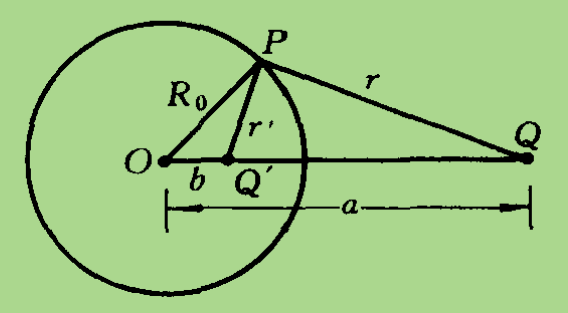
\includegraphics[width=8cm]{figure2-1.png}
        \caption{导体球镜像电荷法示意图}
        \label{figure2.1}
    \end{figure}
    关键是选择镜像电荷$Q^{\prime}$大小和位置使得球面上$\varphi=0$满足
    \begin{equation}
        \frac{Q}{r} + \frac{Q^{\prime}}{r^{\prime}} = 0
    \end{equation}

\noindent 其中,$r = |QP|,\ r^{\prime} = |Q^{\prime} P|$.对任意一点得到$\frac{r^{\prime}}{r} = C$,取$\triangle OQ^{\prime}P \sim \triangle OPQ$,可以满足这个条件,由此可以确定假象电荷的位置和大小
\begin{equation}
    \left \{ \begin{aligned}
        &b = \frac{R_0^2}{a} \\ 
        &Q^{\prime} = - \frac{R_0}{a} Q
    \end{aligned} \right.
\end{equation}

    \subsection{格林函数}
    格林函数法用以求解较为普通的边值问题:\red{对于给定V内电荷分布$\rho$和V的边界S上各点的$\phi_S$或电场法向向量$\frac{\partial \phi}{\partial n}|_S$,求V内各点电势}。

    一样分为两类,所规定的格林函数的边界条件为
    \begin{equation}
        \varphi|_S = 0 \qquad \frac{\partial \varphi}{\partial n}|S = - \frac{1}{\varepsilon_0 S} \label{equ2.1}
    \end{equation}

\noindent 需要注意的是,格林函数本质上是一个假想的由点电荷产生的势,但给定边界条件可得其表达式。利用其与待求势之间耦合并利用其表达式与边界条件便可求出待求势的表达式。格林函数的边界条件原则上可以任意取,但我们取最易于计算的\autoref{equ2.1},并注意与待求势相区分。

    \subsubsection{几种常用的格林函数}
    对于格林函数的形式,列举下面几个常用的
    \paragraph{无界空间} 
    无界空间的格林函数通过镜像法得到
    \begin{equation}
        \varphi(x) = \frac{1}{4 \pi \varepsilon_0 r}
    \end{equation}
\noindent 其中,$r = \sqrt{(x-x^{\prime})^2 + (y-y^{\prime})^2 +(z-z^{\prime})^2}$.

    \paragraph{上半空间}
    上半空间的格林函数对于不同的边界条件形式不同
    \begin{equation}
        G(x,x^{\prime}) = \frac{1}{4 \pi \varepsilon_0} \left(\frac{1}{r} \pm \frac{1}{r^{\prime}}\right)
    \end{equation}
    
\noindent 其中,$r= \sqrt{(x-x^{\prime})^2 + (y-y^{\prime})^2 +(z-z^{\prime})^2}$,$r^{\prime}= \sqrt{(x-x^{\prime})^2 + (y-y^{\prime})^2 +(z+z^{\prime})^2}$. 负号对应于第一类边界条件(边界为等势面,和无穷远处连上,电势为0),正号对应第二类(边界趋向于无穷大,法向导数趋向于0)。

    \paragraph{球外空间}
    还是利用镜像法得到,具体推导可见上一小节。注意待求区域是在球\red{外}。结果如下
    \begin{equation}
        G(\vec{x},\vec{x}^{\prime}) = \frac{1}{4 \pi \varepsilon_0}\left[\frac{1}{\sqrt{R^2 + R^{\prime 2} - 2 R R^{\prime} \cos \alpha}} - \frac{1}{\sqrt{\left(\frac{R R^{\prime}}{R_0}\right) + R_0^2 - 2 R R^{\prime} \cos \alpha}}\right]
    \end{equation}

    \subsubsection{格林公式与边值问题的解}
    先考虑第一类,留意我们现在有哪些已知量,然后运用格林公式将格林函数的问题和待求势能的问题结合起来,用已知量推未知量。

    存在格林公式
    \begin{equation}
        \int_V (\psi \nabla^2 \varphi - \varphi - \nabla^2 \psi)\dif V = \oint_S \left(\psi \frac{\partial \varphi}{\partial n} - \varphi \frac{\partial \psi}{\partial n}\right) \dif S
    \end{equation}

\noindent 为了方便起见(因为最后想用不带撇的量表示场点),所以交换$x \leftrightarrow x^{\prime}$. 由于上式是普遍的,令$\psi$为格林函数,令$\varphi$为待求势,得到
\begin{equation}
    \begin{aligned}
        &\int_{V}\left[G\left(\vec{x}^{\prime}, \vec{x}\right) \nabla^{\prime 2} \varphi\left(\vec{x}^{\prime}\right)-\varphi\left(\vec{x}^{\prime}\right) \nabla^{\prime 2} G\left(\vec{x}^{\prime}, \vec{x}\right)\right] d V^{\prime}\\
        &=\oint_{S}\left[G\left(\vec{x}^{\prime}, \vec{x}\right) \frac{\partial \varphi\left(\vec{x}^{\prime}\right)}{\partial n^{\prime}}-\varphi\left(\vec{x}^{\prime}\right) \frac{\partial}{\partial n^{\prime}} G\left(\vec{x}^{\prime}, \vec{x}\right)\right] \mathrm{d} S^{\prime}
        \end{aligned}
\end{equation}

\noindent 由于$\nabla^2 G(\vec{x},\vec{x}^{\prime}) = \frac{1}{\varepsilon_0} \delta(x^{\prime}-x)$,并考虑边界条件
\begin{equation}
    G(\vec{x}^{\prime},\vec{x})|_S = 0
\end{equation}

\noindent 得到 
\begin{equation}
    \varphi(\vec{x}) = \int_V G(\vec{x}^{\prime},\vec{x})\rho(\vec{x}^{\prime})\dif V^{\prime} - \varepsilon_0 \oint_S \varphi(\vec{x}^{\prime})\frac{\partial}{\partial n} G(\vec{x}^{\prime},\vec{x})\dif S
\end{equation}

    对于第二类边界条件,由于(注意这时$G|_S$不一定成立)
    \begin{equation}
        \frac{\partial G(\vec{x}^{\prime}}{\partial n^{\prime}}|_S = - \frac{1}{\varepsilon_0 S}
    \end{equation}

\noindent 所以
\begin{equation}
    \begin{aligned}
        \varphi(\vec{x})=& \int_{V} G\left(\vec{x}^{\prime}, \vec{x}\right) \rho\left(\vec{x}^{\prime}\right) \mathrm{d} V^{\prime} \\
        &+\varepsilon_{0} \oint_{S} G\left(\vec{x}^{\prime}, \vec{x}\right) \frac{\partial \varphi\left(\vec{x}^{\prime}\right)}{\partial n^{\prime}} d S^{\prime}+\langle\varphi\rangle_{S}
        \end{aligned}
\end{equation}

\noindent 其中$\langle\varphi\rangle_{S}$为再边界上的平均值,作为常数,求不到问题也不大。

    补充通过作用量原理得到运动方程。首先再静电场中的作用量为
    \begin{equation}
        I = \int_V \left(- \frac{1}{2} \nabla \varphi \nabla \varphi + \frac{\rho}{\varepsilon}\varphi\right)\dif V + \oint_S \frac{b}{2} \varphi^2 \dif S
    \end{equation}

\noindent 通过$\delta I =0$可以得到静电场下的运动方程和边界条件
\begin{equation}
    \left\{\begin{aligned}
        &\nabla^2 \varphi = - \frac{\rho }{\varepsilon}\\
        & \left\{\begin{aligned}
            &\delta \varphi = 0 \\
            &\partial_n \varphi = b \varphi
        \end{aligned}\right.
    \end{aligned}\right.
\end{equation}

    \subsection{电多极矩}
    \subsubsection{电势的多级展开}
    真空中给定电荷密度$\rho(\vec{x}^{\prime})$激发的电势为
    \begin{equation}
        \varphi(\vec{x}) = \int \frac{\rho(\vec{x}^{\prime}) \dif V^{\prime}}{4 \pi \varepsilon_0 r} \qquad r = |\vec{x} - \vec{x}^{\prime}|
    \end{equation}

\noindent 当r远大于电荷系统线度l的时候,可以将其表示为$\frac{l}{r}$的展开式。由于对$f(\vec{x}- \vec{x}^{\prime})$在$\vec{x}=0$点附近对$\vec{x}^{\prime}$展开得到
\begin{equation}
    \begin{aligned}
        f\left(\vec{x}-\vec{x}^{\prime}\right) &=f(\vec{x})-\sum_{i=1}^{3} x_i^{\prime} \frac{\partial}{\partial x_i} f(\vec{x})+\frac{1}{2 !} \sum_{i, j} x_i^{\prime} x_j^{\prime} \frac{\partial^{2}}{\partial x_i \partial x_j} f(\vec{x})+\cdots \\
        &=f(\vec{x})-\vec{x}^{\prime} \cdot \nabla f(\vec{x})+\frac{1}{2 !}\left(\vec{x}^{\prime} \cdot \nabla\right)^{2} f(\vec{x})+\cdots
        \end{aligned}
\end{equation}

\noindent 用$f\left(\vec{x}-\vec{x}^{\prime}\right) = \frac{1}{r}$代入得到
\begin{equation}
    \begin{aligned}
        \varphi(\vec{x})=& \frac{1}{4 \pi \varepsilon_{0}} \int_{V} \rho\left(\vec{x}^{\prime}\right)\left[\frac{1}{R}-\vec{x}^{\prime} \cdot \nabla \frac{1}{R}+\frac{1}{2 !} \sum_{i, j} x_i^{\prime} \vec{x}^{\prime} \frac{\partial^{2}}{\partial x_i \partial x_j} \frac{1}{R}+\cdots\right] \mathrm{d} V^{\prime}
        \end{aligned}
\end{equation}

    令总电荷$Q = \int_V \rho(\vec{x}^{\prime}) \dif V^{\prime}$,总电偶极矩$\vec{P} = \int_V \rho(\vec{x}^{\prime}) x^{\prime} \dif V^{\prime}$和总电四极矩$\mathscr{L}_{ij} = \int_V 3 x_i^{\prime} y_j^{\prime} \rho(\vec{x}^{\prime}) \dif V^{\prime}$可以得到
    \begin{equation}
        \varphi(\vec{x})=\frac{1}{4 \pi \varepsilon_{0}}\left[\frac{Q}{R}-\vec{P} \cdot \nabla \frac{1}{R}+\frac{1}{6} \sum_{i, j} \mathscr{L}_{i j} \frac{\partial^{2}}{\partial x_i \partial x_j} \frac{1}{R}+\cdots\right]\label{equ2.2}
    \end{equation}

    \subsubsection{电多极矩}
    对于\autoref{equ2.2},第一项便是在原点点电荷的电势,可见零阶近似项是平庸的,就是点电荷模型;第二项可写作
    \begin{equation}
        \varphi^{(1)} = - \frac{1}{4 \pi \varepsilon_0} \vec{P} \cdot \nabla \frac{1}{R} = \frac{\vec{P} \cdot \vec{R}}{4 \pi \varepsilon_0 R^3}
    \end{equation}

\noindent 是电偶极矩产生的电势。注意,\red{只有对原点不对称的电荷分布才有电偶极矩}。

    对于第三项
    \begin{equation}
        \varphi^{(2)} = \frac{1}{4 \pi \varepsilon_0} \frac{1}{6} \mathscr{L}_{ij} \frac{\partial^2}{\partial x_i \partial x_y} \frac{1}{R}
    \end{equation}

\noindent 是电四极矩产生的电势。这是一个对称张量,具有六个分量但只有5个独立自由度,这是由于
\begin{equation}
    \delta_{ij} \frac{\partial^2}{\partial x_i \partial x_j} \frac{1}{R} = 0
\end{equation}

\noindent 故可将电偶极矩重新定义(这也是更为常用的)
\begin{equation}
    \mathscr{L}_{ij} = \int \left(3 x_i^{\prime} 3 x_j^{\prime} - r^{\prime 2} \delta_{ij}\right) \rho(\vec{x}^{\prime}) \dif V^{\prime}
\end{equation}

\noindent 第三项展开形式不变,但有
\begin{equation}
    \mathscr{L}_{11}+ \mathscr{L}_{22} + \mathscr{L}_{33} = 0
\end{equation}

\noindent 减少了一个独立变量。

    对于球对称电荷分布,有下面两个关系
    \begin{equation}
        \left \{ \begin{aligned}
            &\mathscr{L}_{11} = \mathscr{L}_{22} =\mathscr{L}_{33} = 0 \\
            &\mathscr{L}_{12} = \mathscr{L}_{23} =\mathscr{L}_{31} = 0
        \end{aligned} \right.
    \end{equation}

\noindent 所以没有电四极矩。这是普遍的,对于球对称电荷分布,无论在哪个坐标系下都有同样的结论。电四极矩因此可用以描写对于球状的偏离程度。

    \subsubsection{电荷体系在外电场中的能量}
    电荷体系在外电场中的能量表达式为
    \begin{equation}
        W = \int \rho \varphi_e \dif V 
    \end{equation}

\noindent 其中$\varphi_e$为外电场电势。

    设电荷分布位于小区域内,套路,把$\varphi_e(\vec{x})$对原点展开,得到(\red{注意,从这里开始为了简便起见,有些地方会省略求和符号,但都是符合爱因斯坦求和规则的,请注意分辨}
    \begin{equation}
        \varphi_e(\vec{x}) = \varphi_e(0) + x_i \frac{\partial}{\partial x_i} \varphi_e(0) + \frac{1}{2!} x_i x_j \frac{\partial^2}{\partial x_i \partial x_j} \varphi_e(0) + \cdots 
    \end{equation}

\noindent 所以 
\begin{equation}
    W = Q \varphi_e + \vec{P} \cdot \nabla \varphi_e(0) + \frac{1}{6} \mathscr{L}_{ij} \frac{\partial}{\partial x_i x_j} \varphi_e(0) + \cdots 
\end{equation}

\noindent 其中第一、二、三项分别是点电荷、偶极场和电四极子在外电场中的能量。

    补充偶极子在外电场中的受力情况
    \begin{equation}
        \left \{ \begin{aligned}
            &\vec{F} = - \nabla W = \nabla(\vec{P} \cdot \vec{E}_e) = \vec{P} \cdot \nabla \vec{E}_e \\ 
            &L_{\theta} = - \frac{\partial W^{(1)}}{\partial \theta} = \frac{\partial}{\partial \theta}(P E_e \cos \theta) = - P E_e \sin \theta 
        \end{aligned} \right.
    \end{equation}

\noindent 由此可见,只有在非均匀场中电四极子的能量不为0.

    \section{静磁场}
    \subsection{矢势}
    定义矢势
    \begin{equation}
        \vec{B} = \nabla \times \vec{A}
    \end{equation}

\noindent 物理意义很明确:对一个封闭曲面的磁场的积分(磁通量)等于这个曲面的边界的矢势的积分。曲面的信息因此为边界所确定,同时考虑两个有着共同边界的面,容易知道两个共同边界的面的磁通量之和为零,这是对磁场的\textbf{无源性}的直观理解。

    \subsubsection{微分方程}
    矢势的定义只有一个约束,而对于一个三维矢量场来说需要两个约束(散度和旋度)才能够完全确定,这带来了任意性。可加上辅助条件,比较常用的有两种:库伦规范和洛伦兹规范。这里暂且只提及库伦规范。
    \paragraph{库伦规范}
    \begin{equation}
        \nabla \cdot  \vec{A} = 0
    \end{equation}

\noindent 在这种情况下,才存在
\begin{equation}
    \nabla^2 \vec{A} = \mu \vec{J}
\end{equation}

    这种情况下的矢势无疑是令人愉悦的(当也给了老师出题的可能...),事实上,我们总可以将其他的矢势改写成这种情况下的矢势。假设存在
    \begin{equation}
        \nabla \cdot \vec{A} = u \ne 0
    \end{equation}

\noindent 令$\vec{A}^{\prime} = \vec{A} + \nabla \varphi$使得$\nabla \cdot \vec{A}^{\prime} = 0$,则存在 
\begin{equation}
    \nabla^2 \varphi = - u
\end{equation}

\noindent 由此解出$\varphi$从而得到令人愉悦的矢势。在矢势是令人愉悦的时候,仿照静电场的运动方程得到特解
\begin{equation}
    \vec{A}(\vec{x}) = \frac{\mu}{4 \pi} \int \frac{\vec{J}(\vec{x}^{\prime}) \dif V^{\prime}}{r}
\end{equation}

\noindent 其中,$\vec{x}^{\prime}$是源点,$\vec{x}$是场点,$r = |\vec{x}^{\prime} - \vec{x}|$.

    \subsubsection{矢势边值关系}
    对应于如下两条边值关系
    \begin{equation}
        \left \{ \begin{aligned}
            &\vec{n} \cdot (\vec{B}_2 - \vec{B}_1) = 0 \\ 
            &\vec{n} \times (\vec{H}_2 - \vec{H}_1) = \vec{a}
        \end{aligned} \right.
    \end{equation}

\noindent 因此,在线性介质中,可以得到
\begin{equation}
    A_{2t} = A_{1t}
\end{equation}

\noindent 再考虑库伦规范的话,可以发现矢势的法向向量也是连续的,很显然,这意味着
\begin{equation}
    \vec{A}_2 =\vec{A}_1
\end{equation}

\noindent 这是一个令人无比愉悦的结果。

    \subsubsection{静磁场能量}
    对于静磁场能量
    \begin{equation}
        W = \frac{1}{2} \int \vec{B} \cdot \vec{H} \dif V
    \end{equation}

\noindent 改写成矢势形式得到
\begin{equation}
    \vec{B} \cdot \vec{H} = \nabla \cdot (\vec{A} \times \vec{H}) + \vec{A} \cdot \vec{J}
\end{equation}

\noindent 第一项在全空间积分时会趋于零,则
\begin{equation}
    W = \frac{1}{2} \int \vec{A} \cdot \vec{J} \dif V
\end{equation}

\noindent 注意和电场能量一样,此公式对全空间有效,故不能将$\frac{1}{2} \vec{A} \cdot \vec{J}$视为磁场能量密度。

    注意,刚才计算的是$\vec{A}$由$\vec{J}$激发的,只有它们两个在自娱自乐,现在我们需要考虑的是,给定某电流分布$\vec{J}$,在给定外磁场中的相互作用能量。不妨令$\vec{A}_e,\vec{J}_e$为外磁场的矢势和电流,则
    \begin{equation}
        W_i = \frac{1}{2} \int (\vec{J} + \vec{J}_e)\cdot (\vec{A} + \vec{A}_e)\dif V
    \end{equation}

\noindent 得到相互作用能
\begin{equation}
    W_i = \frac{1}{2}\int (\vec{J} \cdot \vec{A}_e + \vec{J}_e \cdot \vec{A}) \dif V
\end{equation}

\noindent 上式的两项是相等的——可以将矢势的表达式写出来,便能够看出来了,所以得到
\begin{equation}
    W_i = \int \vec{J} \cdot \vec{A}_e \dif V
\end{equation}

    \subsection{磁标势}
    当存在
    \begin{equation}
        \oint \vec{H} \cdot \dif \vec{l} = 0
    \end{equation}
\noindent 时,意味着该区域内任何回路都不被电流链环,即为无自由电流分布的单连通区域。这时可以引入磁标势
\begin{equation}
    \vec{H} = - \nabla \varphi_m
\end{equation}

\noindent 后面可以仿照静电场的情况进行各种推导。由于我对磁标势没有什么好感,就不多说了。

    \subsection{磁多极距}
    \subsubsection{矢势的多级展开}
    对于矢势
    \begin{equation}
        \vec{A}(\vec{x})= \frac{\mu_0}{4 \pi} \int \frac{\vec{J}(\vec{x}^{\prime}) \dif V^{\prime}}{r} 
    \end{equation}

\noindent 考虑电流分布于小区域的情况,远场下,得到多级展开
\begin{equation}
    \vec{A} (\vec{x}) = \frac{\mu_0}{4 \pi }\int \vec{J}(\vec{x}^{\prime}) \left[\frac{1}{R} - \vec{x}^{\prime} \cdot \nabla \frac{1}{R} + \frac{1}{2!}x_j^{\prime} x_i^{\prime} \frac{\partial^2 }{\partial x_i \partial x_j} + \cdots\right] \dif V^{\prime}
\end{equation}

    第一项,由于可将电流分为许多闭合流管,得到
    \begin{equation}
        \int \vec{J}(\vec{x}^{\prime}) \dif V^{\prime} = \oint I \dif \vec{l} = I \oint \dif \vec{l} = 0
    \end{equation}

\noindent 不含磁单极项。对于第二项,同样将电流分为闭合流管,得到
\begin{equation}
    \vec{A}^{(1)} = \frac{\mu_0}{4 \pi R^3}\frac{I}{2} \oint (\vec{x}^{\prime} \times \dif \vec{l})\times \vec{R} = \frac{\mu_0}{4 \pi} \frac{\vec{m} \times \vec{R}}{R^3}
\end{equation}

\noindent 式中$\vec{m} = \frac{I}{2} \oint \vec{x}^{\prime} \times \dif \vec{l}^{\prime}$称为电流线圈的磁矩。

    令$I \dif \vec{l}^{\prime} \rightarrow \vec{J} \dif V^{\prime}$得到
    \begin{equation}
        \vec{m} = \frac{1}{2} \int \vec{x}^{\prime} \times \vec{J}(\vec{x}^{\prime}) \dif V^{\prime}
    \end{equation}

\noindent 对于一个小线圈,设
\begin{equation}
    \Delta \vec{S} = \frac{1}{2} \oint \vec{x}^{\prime} \times \dif \vec{l}^{\prime}
\end{equation}

\noindent 因此
\begin{equation}
    \vec{m} = \vec{I} \Delta \vec{S}
\end{equation}

    \subsubsection{磁偶极矩的场}
    对矢势展开的第二项可以得到
    \begin{equation}
        \vec{B}^{(1)} = \nabla \times \vec{A}^{(1)} = \frac{\mu_0}{4 \pi } \left[(\nabla \cdot \frac{\vec{R}}{R^3})\vec{m} - (\vec{m} \cdot \nabla) \frac{\vec{R}}{R^3}\right]
    \end{equation}

\noindent 由于当$R \ne 0$时, 
\begin{equation}
    \nabla \left(\frac{\vec{R}}{R^3}\right) = -\nabla^2 \frac{1}{R} = 0
\end{equation}

\noindent 故
\begin{equation}
    B^{(1)} = - \frac{\mu_0}{4 \pi} (\vec{m} \cdot \nabla) \frac{\vec{R}}{R^3}
\end{equation}

    \subsubsection{小区域内电流分布在外磁场中的能量}
    首先利用之前得到的能量公式得到
    \begin{equation}
        W = \int \vec{J} \cdot \vec{A}_e \dif V
    \end{equation}

\noindent 对于载有电流$I$的线圈得到
\begin{equation}
    W = I \oint_L \vec{A}_e \cdot \dif \vec{l} = I \int_S \vec{B}_e \cdot \dif \vec{S} = I \phi_0
\end{equation}

\noindent 若区域线度小于磁场发生显著变化的线度,则可以把$\vec{B}_e(x)$在原点领域展开,得到第一项
\begin{equation}
    W^{(1)} = I \vec{B}_0 \int \dif \vec{S} = \vec{m} \cdot \vec{B}_e(0)
\end{equation}

    这里出现个问题,结果和电偶极子的能量$W = - \vec{P} \cdot \vec{E}_e$反向。这是由于我们假设线圈上电流I以及产生外磁场的电流$I_e$是不变的,但实际上要保持它们不变需要外接电源,而电源供能为
    \begin{equation}
        \delta W_s = I \delta \Phi_e + I_e \delta \Phi = 2 \delta W
    \end{equation}

\noindent 其中$\delta W$为磁能的总该变量。现在体系中其实包括有相互作用的三部分:外电源、电磁场以及两个线圈上的电流,能量守恒的完整式子如下
\begin{equation}
    \delta W_s = \delta W + \delta A
\end{equation}

\noindent 其中$\delta A$是对线圈做的功,它等于磁场的增量,而不是如一般情况下(没有外部势力作用)是磁场的变化量的相反数。所以
\begin{equation}
    U = -W = - \int \vec{J} \cdot \vec{A}_e \dif V = - \vec{m} \cdot \vec{B}_e
\end{equation}

\noindent 和电场情况完全对应。

    补充受力情况:
    \begin{equation}
        \vec{F} = - \nabla U = \vec{m} \cdot \nabla \vec{B}e
    \end{equation}

\noindent 这是由于$\nabla \times \vec{B}_e =0$

    力矩为
    \begin{equation}
        \vec{L} = \vec{m} \times \vec{B}_e
    \end{equation}

    \section{电磁波的传播}
    电磁波的传播主要由麦克斯韦方程组和边值关系描述。麦克斯韦方程组形式如下
    \begin{equation}
        \left\{ \begin{aligned}
            \nabla \times \vec{E} &= - \frac{\partial \vec{B}}{\partial t}\\
            \nabla \times \vec{B} &= \frac{\partial \vec{D}}{\partial t} + \vec{J}\\
            \nabla \cdot \vec{D} &=\rho \\
            \nabla \cdot \vec{B} &=0
        \end{aligned}
        \right.
    \end{equation}

    边值关系可以通过麦克斯韦关系得到(不同角标表示不同的介质)
    \begin{equation}
        \begin{aligned}
            \vec{n} \times (\vec{E}_2 - \vec{E}_1) &=0 \\
            \vec{n} \times (\vec{H}_2 - \vec{H}_1) &=\vec{a} \\
            \vec{n} \cdot (\vec{D}_2 - \vec{D}_1) &=\sigma \\
            \vec{n} \cdot (\vec{B}_2 - \vec{B}_1) &=0 
        \end{aligned}\label{equ4.2}
    \end{equation}

    \subsection{平面电磁波}
    现在考虑自由空间下的麦克斯韦关系。在自由空间中,$\rho=0$和$\vec{J} = 0$,所以
    \begin{equation}
    \left\{ \begin{aligned}
        \nabla \times \vec{E} &= - \frac{\partial \vec{B}}{\partial t}\\
        \nabla \times \vec{B} &= \frac{\partial \vec{D}}{\partial t}\\
        \nabla \cdot \vec{D} &=0 \\
        \nabla \cdot \vec{B} &=0
    \end{aligned}
    \right.
    \end{equation}

    令$c = \frac{1}{\sqrt{\varepsilon \mu}}$,得到电场和磁场的微分方程
    \begin{equation}
        \left\{\begin{aligned}
            \nabla^2 \vec{E} - \frac{1}{c^2} \frac{\partial^2 \vec{E}}{\partial t^2} &=0 \\
            \nabla^2 \vec{B} - \frac{1}{c^2} \frac{\partial^2 \vec{B}}{\partial t^2} &=0
        \end{aligned}\right. \label{equ4.1}
    \end{equation}
\noindent 形式如\autoref{equ4.1}的被称为\textbf{波动方程},由电磁场的波动方程可以得到各式各样的电磁波解(在真空条件下)。
    现在考虑介质中的情况。在介质中需要给出电磁场和辅助场之间的关系,即
    \begin{equation}
        \begin{aligned}
            \vec{D} &= \vec{\varepsilon} \vec{E} \\
            \vec{B} &= \vec{\mu} \vec{D}
        \end{aligned}
    \end{equation}

\noindent 其中的$\vec{\varepsilon}$和$\vec{\mu}$被称为\textbf{电介质常数}和\textbf{磁介质常数},可以是标量函数(包括常数)和二阶张量。

    \subsubsection{时谐电磁波}
    现在考虑单频电磁波,此时电介质常数和磁介质常数均为常数(叫作常数,实则是和频率相关的),电场和磁场的解形式如下
    \begin{equation}
        \left \{ \begin{aligned}
            \vec{E}(x,t) &= \vec{E} e^{-i\omega t} \\
            \vec{B}(x,t) &= \vec{B} e^{-i \omega t}
        \end{aligned} \right.
    \end{equation}

\noindent 以电场为例,考虑到$\nabla \times (\nabla \times \vec{E}) = \omega^2 \mu \varepsilon \vec{E}$,可以得到
    \begin{equation}
        \nabla^2 \vec{E} + k^2 \vec{E} = 0
    \end{equation}

\noindent 这个方程被称为\textbf{亥姆霍兹方程},对于电场和磁场均适用,其中$k = \omega \sqrt{\mu \varepsilon}$,但要注意需要加上条件$\nabla \cdot \vec{E} = 0$才能和麦克斯韦方程(真空条件下)等价。(时谐情况下由于辅助场和电磁场之前的关系是简单的线性关系,等于增加了约束,麦克斯韦方程组自由度下降为2)
    一般情况下先利用亥姆霍兹方程求出电场,然后利用电场和磁场之间的关系求出磁场
    \begin{equation}
        \vec{B} = - \frac{i}{\omega} \nabla \times \vec{E} = - \frac{i}{k} \sqrt{\mu \varepsilon} \nabla \times \vec{E}
    \end{equation}

    \subsubsection{平面电磁波}
    全空间的时谐电磁波的形式为平面电磁波,若沿x轴传播,则同相位点正好位于同一平面(yz平面),形式如下
    \begin{equation}
        \vec{E}(x,t) = \vec{E_0} e^{i(kx-\omega t)}
    \end{equation}

\noindent 一般坐标系下,由于传播方向和基矢不一定平行和垂直,这个时候电场方程为
\begin{equation}
    \vec{E}(x,t) = \vec{E_0} e^{i(\vec{k} \cdot \vec{x}-\omega t)}
\end{equation}

    \subsubsection{能量和能流}
    能量和能流(密度)的公式如下
    \begin{equation}
        \begin{aligned}
            w &= \frac{1}{2}(\vec{E} \cdot \vec{D} + \vec{H} \cdot \vec{B}) = \frac{1}{2} (\varepsilon E^2 + \frac{1}{\mu} B^2) \\
            \vec{S} &= \vec{E} \times \vec{H} = \sqrt{\frac{\varepsilon}{\mu}} \vec{E} \times (\vec{n} \times \vec{E}) = \sqrt{\frac{\varepsilon}{\mu}} E^2 \vec{n} = v \omega \vec{n}
        \end{aligned}
    \end{equation}
\noindent 其中,$v$为相速度。

    由于能量和能流密度是关于场强的二次式,计算瞬时值时不应该将复数直接代入,而应该只代入实数部分。对于二次式求平均采用以下公式
    \begin{equation}
        \begin{aligned}
            \overline{fg} &= \frac{1}{2} \operatorname{Re}(f^{*} g) \\
            \overline{f \times g} &= \frac{1}{2} \operatorname{Re}(f^{*} \times g)
        \end{aligned}
    \end{equation}

    \subsection{电磁波的反射和折射}
    \subsubsection{方向关系}
    电磁波的反射和折射依据的是边值关系\autoref{equ4.2}. 代入平面电磁波的表达式后可以发现在分界面上(z=0)
    \begin{equation}
        \vec{n} \times\left(\vec{E}_{0} \mathrm{e}^{\mathrm{i} \vec{k} \cdot \vec{x}}+\vec{E}_{0}^{\prime} \mathrm{e}^{\mathrm{i} \vec{k} \cdot \vec{x}}\right)=\vec{n} \times \vec{E}_{0}^{\prime \prime} \mathrm{e}^{\mathrm{i} \vec{k}^{\prime \prime} \cdot \vec{x}}
    \end{equation}

\noindent 要使该式在分界面上处处成立,即要求
\begin{equation}
    \vec{k} \cdot \vec{x}=\vec{k}^{\prime} \cdot \vec{x}=\vec{k}^{\prime \prime} \cdot \vec{x} \qquad (z=0)
\end{equation}

\noindent 所以
\begin{equation}
    k_x = k_x^{\prime} = k_x^{\prime \prime} \qquad k_y=k_y^{\prime} = k_y^{\prime \prime} \label{equ4.3}
\end{equation}

\noindent 令入射面位于xz平面,由\autoref{equ4.3}第二式可以得到入射、折射和反射电磁波\textbf{共面}。

    结合$k= \frac{\omega}{v}$,$v = \frac{c}{\sqrt{\mu \varepsilon}}$和$n = \frac{c}{v}$可以得到
    \begin{equation}
        \begin{aligned}
            \frac{\sin \theta}{\sin \theta^{\prime}} &= \frac{n_2}{n_1} \\
            \frac{\sin \theta}{\sin \theta^{\prime \prime}} &=\frac{n_3}{n_1}
        \end{aligned}
    \end{equation}

    \subsubsection{幅值关系——菲涅耳公式}
    \begin{itemize}
        \item $\overline{E} \perp$入射面
        \begin{equation}
            \left \{ \begin{aligned}
                &\vec{E} + \vec{E}^{\prime} = \vec{E}^{\prime \prime} \\
                &\vec{H} \cos \theta - \vec{H}^{\prime} \cos \theta^{\prime} = \vec{H}^{\prime \prime} \cos \theta^{\prime \prime}
            \end{aligned} \right.
        \end{equation}

        \item $\overline{E} \parallel$入射面
        \begin{equation}
            \left \{ \begin{aligned}
                &\vec{E} \cos \theta - \vec{E}^{\prime} \cos \theta^{\prime} = \vec{E}^{\prime \prime} \cos \theta^{\prime \prime} \\
                &\vec{H} + \vec{H}^{\prime} = \vec{H}^{\prime \prime}
            \end{aligned} \right.
        \end{equation}
    \end{itemize}

    \subsubsection{全反射}
    当电磁波从介密介质向介疏介质倾斜射入时,存在大于一个角使得电磁波完全反射的情况,这个时候$\sin \theta > n_{21}$和$k_x^{\prime \prime} > k^{\prime}$,故得到
    \begin{equation}
        k_z^{\prime \prime} = \sqrt{k^{\prime \prime 2} - k^{\prime \prime 2}_x} = ik \sqrt{\sin^2 \theta - n_{21}^2} 
    \end{equation}

\noindent 这时若令$k_z^{\prime \prime} = i \kappa$可以得到
\begin{equation}
    \vec{E}^{\prime \prime} = \vec{E}_0^{\prime \prime} e^{- \kappa z} e^{i(k^{\prime \prime}_x x - \omega t)}
\end{equation}
\noindent 由于衰减项的存在,这个波只会存在于$z>0$的波长量级的空间中
\begin{equation}
    d \sim \kappa^{-1} = \frac{1}{k \sqrt{\sin^2 \theta - n_{21}^2}} = \frac{\lambda_1}{2 \pi \sqrt{\sin^2 \theta - n_{21}^2}}
\end{equation}

    利用$\vec{H} = - \frac{i}{k} \sqrt{\mu \varepsilon} \nabla \times \vec{E}$,考虑垂直入射的情况($\vec{E}= E_y \hat{j}$),得到磁场
    \begin{equation}
    \begin{array}{l}{H_{z}^{\prime \prime}=\sqrt{\frac{\varepsilon_{2}}{\mu_{2}}} \frac{k_{x}^{\prime \prime}}{k^{\prime \prime}} E_{y}^{\prime \prime}=\sqrt{\frac{\varepsilon_{2}}{\mu_{2}} \sin \theta} E^{\prime \prime}} \\ {H_{x}^{\prime \prime}=-\sqrt{\frac{\varepsilon_{2}}{\mu_{2}}} \frac{k_{z}^{\prime \prime}}{k^{\prime \prime}} E_{y}^{\prime \prime}=-i \sqrt{\frac{\varepsilon_{2}}{\mu_{2}}} \sqrt{\frac{\sin ^{2} \theta}{n_{21}^{2}}-1} E^{\prime \prime}}\end{array}
    \end{equation}

\noindent $H_z^{\prime \prime}$与$E^{\prime \prime}$同相,但$H_x^{\prime \prime }$与$E^{\prime \prime}$有$90^{\circ}$的相位差。

    折射波平均能流密度为
    \begin{equation}
    \begin{array}{l}{\bar{S}_{x}^{\prime \prime}=\frac{1}{2} \operatorname{Re}\left(E_{y}^{\prime \prime *} H_{z}^{\prime \prime}\right)=\frac{1}{2} \sqrt{\frac{\varepsilon_{2}}{\mu_{2}}}\left|E_{0}^{\prime \prime}\right|^{2} \mathrm{e}^{-2 \kappa z }}\frac{\sin}{n_{21}} \\ {\bar{S}_{z}^{\prime \prime}=-\frac{1}{2} \operatorname{Re}\left(E_{y}^{\prime \prime *} H_{x}^{\prime \prime}\right)=0}\end{array}
    \end{equation}

\noindent 由此,折射波平均能流只有x分量,沿z轴方向投入第二介质的平均能流密度为零。

    在全反射情况下,入射波和反射波振幅相等,但相位不同,因而瞬时能流值是不同的。由此可见,在全反射过程中第二介质是起作用的。在半周内,电磁能量透入第二介质,在洁面附近薄层内储存起来,在另一半周内,该能量释放出来变为反射波能量。

    \subsection{导体存在时电磁波的传播}
    导体中存在自由电子,在电磁波电场地作用下,自由电子运动形成传导电流,由电流产生的焦耳热使电磁波能量不断损耗,所以在导体内部地电磁波是一种衰减波,在传播过程中,电磁能量转化为热量。导体内电磁波的传播过程是交变电磁场与自由电子运动相互制约的过程,这种相互作用决定导体内电磁波的存在形式。

    \subsubsection{导体内的自由电荷分布}
    考虑在导体内部某区域内的自由电荷分布,假设其密度为$\rho$. 这电荷密度分布激发电场$\vec{E}$
    \begin{equation}
        \varepsilon \nabla \cdot \vec{E} = \rho 
    \end{equation}

\noindent 在电场$\vec{E}$作用下,导体内引起传导电流$\vec{J}$,由欧姆定律得到
\begin{equation}
    \vec{J}= \sigma \vec{E}
\end{equation}
\noindent 比较后可知,当导体内某处有电荷密度时,就会有电流从该处流出,从物理上看这是明显的。由于电荷外流,每一体元内地电荷密度减小,可以得到
\begin{equation}
    \rho(t) = \rho_0 e^{-\frac{\sigma}{\varepsilon}t} 
\end{equation}

    取特征时间——电荷密度减小为原来的$\frac{1}{e}$的时间
    \begin{equation}
        \tau = \frac{\varepsilon}{\sigma}
    \end{equation}
\noindent 良导体条件被定义为电磁波的频率满足$\omega \ll \tau^{-1}$,即
\begin{equation}
    \frac{\sigma}{\varepsilon \omega} \gg 1
\end{equation}

\noindent 此时可以认为内部没有自由电荷分布,电荷只分布于导体表面上。

    \subsubsection{导体内电磁波}
    考虑导体内部的麦克斯韦方程组:$\rho=0, \quad \vec{J} = \sigma \vec{E}$
    \begin{equation}
        \left \{ \begin{array}{l}{\nabla \times \vec{E}=-\frac{\partial \vec{B}}{\partial t}} \\ {\nabla \times \vec{H}=\frac{\partial \vec{D}}{\partial t}+\vec{J}} \\ {\nabla \cdot \vec{D}=0} \\ {\nabla \cdot \vec{B}=0}\end{array} \right.
    \end{equation}
    
\noindent 考虑时谐条件$\vec{D} = \varepsilon \vec{E}, \quad \vec{H} = \frac{\vec{B}}{\mu}$得到
\begin{equation}
    \left \{ \begin{array}{l}{\nabla \times \vec{E}=\mathrm{i} \omega \mu \vec{H}} \\ {\nabla \times \vec{H}=-\mathrm{i} \omega \epsilon \vec{E}+\sigma \vec{E}} \\ {\nabla \cdot \vec{E}=0} \\ {\nabla \cdot \vec{H}=0}\end{array} \right.
\end{equation}

    形式上可引入
    \begin{equation}
        \varepsilon^{\prime} = \varepsilon + i \frac{\sigma}{\omega}
    \end{equation}

\noindent 得到
\begin{equation}
    \nabla \times \vec{H} = -i w \omega \varepsilon^{\prime} \vec{E}
\end{equation}

\noindent 因此求解可以类比绝缘介质中的方程,得到亥姆霍兹方程(只举电场为例)
\begin{equation}
    \left \{ \begin{aligned}
        &\nabla^2 \vec{E} + k^2 \vec{E} = 0 \\
        &k=\omega \sqrt{\mu \varepsilon^{\prime}} 
    \end{aligned} \right.
\end{equation}

    此时$\vec{k}$为一个复数,可写作
    \begin{equation}
        \vec{k} = \vec{\beta}+ i \vec{\alpha}
    \end{equation}

\noindent 其中,$\vec{\beta}$和$\vec{\alpha}$分别被称为\textbf{相位常数}和\textbf{衰减常数}。由此可到的平面波电场解为
\begin{equation}
    \vec{E}(\vec{x},t) = \vec{E_0}e^{-\vec{\alpha} \cdot \vec{x}-\omega t}
\end{equation}

    由于$k^2 = \beta^2 - \alpha^2 + 2 i \vec{\alpha} \cdot \vec{\beta} = \omega^2 \mu (\varepsilon + i \frac{\sigma}{\omega})$,从而得到
    \begin{equation}
        \left \{ \begin{aligned}
            &\beta^2 - \alpha^2 = \omega^2 \mu \varepsilon \\
            & \vec{\alpha} \cdot \vec{\beta} = \frac{1}{2} \omega \mu \sigma 
        \end{aligned} \right.\label{equ4.4}
    \end{equation}

    若导体中波的传播方向为x轴方向,则
    \begin{equation}
        \vec{k} = k_x \hat{i} = \beta_x \hat{i} + i \alpha_x \hat{i}
    \end{equation}

\noindent 由于这是空间中实际存在的可测量的波矢,理应为实数,故$\beta_x = k_x$,$a_x=0$.

    \subsubsection{趋肤效应和穿透深度}
    由于有衰减因子,电磁波只能透入导体表面薄层内。因此,有导体存在时的电磁波传播问题一般是作为边值问题考虑的。电磁波主要是在导体之外地空间或介质中春波,在导体表面上,电磁波与导体中的自由电荷相互作用,引起导体表层的电流,这电流的存在使得电磁波向空间反射,一部分电磁能量透入导体内,形成导体表面薄层内的电磁波,最后通过传导电流把这部分能量耗散为焦耳热。
    
    考虑垂直入射下,电场的表达式为
    \begin{equation}
        \vec{E} = \vec{E_0} e^{-\alpha z} e^{i(\beta z - \omega z)}
    \end{equation}

    由\autoref{equ4.4}可以解出
    \begin{equation}
    \begin{array}{l}{\beta=\omega \sqrt{\mu \epsilon}\left[\frac{1}{2}(\sqrt{1+\frac{\sigma^{2}}{\varepsilon^{2} \omega^{2}}}+1)\right]^{\frac{1}{2}}} \\ {\alpha=\omega \sqrt{\mu \varepsilon}\left[\frac{1}{2}(\sqrt{1+\frac{\sigma^{2}}{\varepsilon^{2} \omega^{2}}}-1)\right]^{\frac{1}{2}}}\end{array}
    \end{equation}

    对于良导体的情况,考虑$k^2$的虚数和实数之比$\frac{\sigma}{\varepsilon \omega} \ll 1$,因而实部可以忽略,得到
    \begin{equation}
        \begin{aligned}
            k^2 &\approx i \omega \mu \sigma \\
            k &\approx \sqrt{i \omega \mu \sigma} \approx \beta + i \alpha
        \end{aligned}
    \end{equation}

\noindent 由此得到
\begin{equation}
    \alpha \approx \beta \approx \sqrt{\frac{\omega \mu \sigma}{2}} \label{equ4.5}
\end{equation}

\noindent 定义波的幅值降低为原来的$\frac{1}{e}$的传播距离称为\textbf{穿透深度}$\delta$:
\begin{equation}
    \delta = \frac{1}{\alpha} = \sqrt{\frac{2}{\omega \mu \sigma}}
\end{equation}
\noindent 可见穿透深度与电导率及频率的平分根成正比。

    利用磁场和电场的关系可到
    \begin{equation}
        \vec{H} = \frac{1}{\omega \mu} \vec{k} \times \vec{E} = \frac{1}{\omega \mu}(\beta + i \alpha) \vec{n} \times \vec{E} \label{equ4.6}
    \end{equation}

\noindent 式中$\vec{n}$为指向导体内部的法线。在良导体内,由于\autoref{equ4.5}可以得到
\begin{equation}
    \vec{H} \approx \sqrt{\frac{\sigma}{\omega \mu}} e^{i \frac{\pi}{4}} \vec{n} \times \vec{E}
\end{equation}

\noindent 容易看出,磁场相位相比电场相位滞后$\frac{\pi}{4}$,且
\begin{equation}
    \sqrt{\frac{\mu}{\varepsilon}} \left|\frac{\vec{H}}{\vec{E}}\right| = \sqrt{\frac{\sigma}{\omega \varepsilon}} \gg 1
\end{equation}

\noindent 因此在金属导体中,相对于真空或绝缘介质来说,磁场远比电场重要,金属内电磁波的能量主要是磁场能量。这是由于电磁波进入金属后激发电流带走电场能量的缘故。

    \subsubsection{导体表面上的反射}
    考虑垂直入射的情况,假设电磁波由真空入射于导体表面,在界面上产生反射波和透入导体内的折射波,根据边值关系
    \begin{equation}
        \begin{aligned}
            E + E^{\prime} &= E^{\prime \prime} \\
            H - H^{\prime}&= H^{\prime \prime}
        \end{aligned}
    \end{equation}
\noindent 在良导体情形,利用\autoref{equ4.6}得到
\begin{equation}
    E - E^{\prime} = \sqrt{\frac{\sigma}{2 \omega \varepsilon_0}}(1+i) E^{\prime \prime}
\end{equation}

\noindent 容易得到
\begin{equation}
    \frac{E^{\prime}}{E}=-\frac{1+i-\sqrt{\frac{2 \omega \varepsilon_{0}}{\sigma}}}{1+i+\sqrt{\frac{2 \omega \varepsilon_{0}}{\sigma}}}
    \end{equation}

\noindent 定义反射系数$R$为反射能流与入射能流之比
\begin{equation}
    R=\left|\frac{E^{\prime}}{E}\right|^{2}=\frac{(1-\sqrt{\frac{2 \omega \varepsilon_{0}}{\sigma}})^{2}+1}{(1+\sqrt{\frac{2 \omega \varepsilon_{0}}{\sigma}})^{2}+1} \approx 1-2 \sqrt{\frac{2 \omega \varepsilon_{0}}{\sigma}}
    \end{equation}

\noindent 由上式可见,电导率越高,则反射系数越接近于1. 对于波长较长的微波或无线电波,反射系数接近于1,只有很小部分电磁能量透入导体内部而被吸收掉,绝大部分能量被反射出去,因此这种情况下往往可以把金属近似看作理想导体。

    \subsection{谐振腔}
    无界空间中电磁波基本的存在形式为平面电磁波,横向振荡,称为横电磁波(TEM)。而根据上节结果,直到电磁波主要是在导体以外的空间或绝缘介质中传播的,只有很小部分电磁能量透入导体表面内。在理想导体($\sigma \to \infty$)极限情形下,导体表面自然构成电磁波存在的边界。这种有界空间中传播的电磁波有本身的特点,下面就来讨论一下这种电磁波。

    \subsubsection{理想导体边界条件}
    实际导体虽然不是理想导体,但是对于一般的金属导体,对无线电波连说,透入其内而损耗的电磁能量一般很小,接近于理想导体。因此,在实际分析问题时,在第一级近似下可以先把金属看作理想导体,然后在第二级近似下再考虑有限电导率引起的损耗。

    考虑边界条件\autoref{equ4.2},取角标1代表理想导体,角标2代表真空或绝缘介质,取法线由导体指向介质中。在理想导体情况下,导体内部没有电磁场,故可取$\vec{E_1} = \vec{H_1} =0$. 略去角标2,有边界条件
    \begin{equation}
        \begin{aligned}
            \vec{n} \times \vec{E} &=0 \\
            \vec{H} = \vec{a}
        \end{aligned}
    \end{equation}

\noindent 由于真空,另外两个条件自然满足。上式中有关磁场的式子反应介质中电磁波的磁场强度与导体表面上高频电流的相互关系。解出介质中电磁波后,由此式可得导体表面电流分布形式。因此,真正制约着电磁波存在的是有关电场的式子。亥姆霍兹方程的解加上条件$\nabla \cdot \vec{E}$,再加上式的边界条件就可以得到该边值问题的解,即该问题中可能存在的电磁波模。对于条件$\nabla \cdot \vec{E}$,在边界处为
\begin{equation}
    \frac{\partial E_n}{\partial n} = 0
\end{equation}

    \newpage
    \subsubsection{谐振腔}
    \begin{wrapfigure}{r}{0.5 \textwidth}
        \centering
        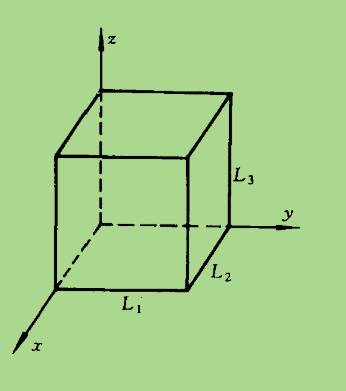
\includegraphics[width=6cm]{figure4-1.png}
        \caption{矩形谐振腔}
        \label{figure4.1}
    \end{wrapfigure}

    考虑矩形谐振腔内的电磁振荡,如\autoref{figure4.1}所示。设$u(x,y,z)$为$\vec{E}$或$\vec{H}$的任一直角分量,有
    \begin{equation}
        \nabla^2 u + k^2 u = 0
    \end{equation}

\noindent 利用分离变量法$u(x,y,z)=X(x)Y(y)Z(z)$可以分解为三个方程
\begin{equation}
\left.\begin{array}{l}{\frac{d^{2} X}{d x^{2}}+k_{x}^{2} X=0} \\ {\frac{d^{2} Y}{d y^{2}}+k_{y}^{2} Y=0} \\ {\frac{d^{2} Z}{d z^{2}}+k_{z}^{2} Z=0}\end{array}\right\}
\end{equation}

\noindent 同时
\begin{equation}
    k_x^2 + k_y^2 +k_z^2 = \omega^2 \mu \varepsilon
\end{equation}

\noindent 考虑边界条件,$\frac{\partial E_n}{\partial n} = 0$,最终得到
\begin{equation}
\begin{array}{l}{E_{x}=A_{1} \cos k_{x} x \sin k_{y} y \sin k_{z} z} \\ {E_{y}=A_{2} \sin k_{x} x \cos k_{y} y \sin k_{z} z} \\ {E_{z}=A_{3} \sin k_{x} x \sin k_{y} y \cos k_{z} z}\end{array} \label{equ4.7}
\end{equation}

\noindent 再考虑$x=L_1,y=L2,z=L_3$的边界条件,得到分立条件
\begin{equation}
    k_x = \frac{m \pi}{L_1}, \quad k_y = \frac{n \pi }{L_2} , \quad k_z = \frac{p \pi }{L_3}
\end{equation}

\noindent $m,n,p$分别代表沿矩形三边所含的半波数目。这三个数最多一个为零,不然场强$\vec{E} = 0$.

    \autoref{equ4.7}式含有三个任意常数,通过方程$\nabla \cdot \vec{E} = 0$,它们之间满足关系
    \begin{equation}
        k_x A_1 + k_y + A_2 + k_z A_3 =0
    \end{equation}

\noindent 因此三个常数只有两个是独立的。对每一组$(m,n,p)$值,有两个独立偏振波模。对此可以这样理解:一个波模意味着一组$(m,n,p)$,而在一个$\vec{A}$空间中存在几个自由度便是几个独立偏振波模。

    谐振频率如下
    \begin{equation}
        \omega_{mnp} = \frac{\pi}{\sqrt{\mu \varepsilon}} \sqrt{\left(\frac{m}{L_1}\right)^2 + \left(\frac{n}{L_2}\right)^2+\left(\frac{p}{L_3}\right)^2}
    \end{equation}

\noindent 这被称为谐振腔的本征频率。

    \subsection{波导}
    \subsubsection{高频电磁能量的传输}
    高频电磁能量的传输与低频相比有显著的不同的特点。在所有情况下,能量都是在场中传播的,在低频情况下,由于场和线路中电荷和电流的关系比较简单,因而场在线路中的作用旺旺可以通过线路的一些参数(电压、电流、电阻、电容和电感等)表示出来。在这种情况下,我们可以用电路方程解决实际问题,而不必直接研究场的分布。但在高频情况下,\textbf{场的波动性显著},集中的电容、电感等概念已经不能使用,而且整个线路上的电流不再是一个与位置无关的量,电压的概念也失去了确切的意义。因此,在高频情况下,电路方程逐渐失效,我们必须直接研究场和线路上的电荷电流的相互作用,解出电磁场,然后才能解决电磁能量传输的问题。

    \subsubsection{矩形波导中的电磁波}
    \begin{wrapfigure}{r}{0.5 \textwidth}
        \centering
        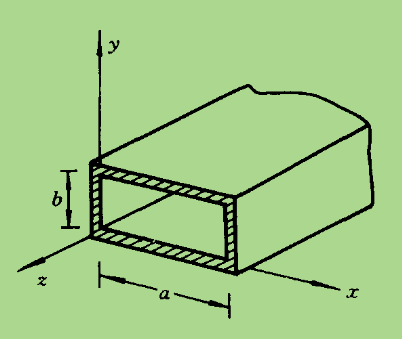
\includegraphics[width=6cm]{figure4-2.png}
        \caption{矩形波导示意图}
        \label{figure4.2}
    \end{wrapfigure}

    考虑\autoref{figure4.2}这样的矩形波导,z轴为传播方向。在一定频率下,管内电磁波是亥姆霍兹方程
    \begin{equation}
        \left \{ \begin{aligned}
            & \nabla^2 \vec{E} + k^2 \vec{E} = 0 \\
            & k = \omega \sqrt{\mu \varepsilon}
        \end{aligned} \right.
    \end{equation}

\noindent 满足条件$\nabla \cdot \vec{E}$的解。此解在管壁上还满足边界条件$\nabla \times \vec{E}$,即电场在管壁上的切向分量为零。

    由于电磁波沿z轴方向传播,它应有传播因子$e^{i k_z z - i \omega t}$,所以可将电场取为
    \begin{equation}
        \vec{E}(x,y,z) = \vec{E}(x,y)e^{i k_z z}
    \end{equation}

\noindent 同样使用分离变量法并利用边值条件,可以得到电场分量为
\begin{equation}
\begin{array}{l}{E_{x}=A_{1} \cos k_{x} x \sin k_{y} y \mathrm{e}^{\mathrm{i} k_{z} z}} \\ {E_{y}=A_{2} \sin k_{x} x \cos k_{y} \mathrm{y} \mathrm{e}^{\mathrm{i} k_{z} z}} \\ {E_{z}=A_{3} \sin k_{x} x \sin k_{y} y \mathrm{e}^{\mathrm{i} k_{z} z}}\end{array}
\end{equation}

\noindent 其中$k_x,k_y$具有如下限制
\begin{equation}
    k_x = \frac{m \pi }{a}, \quad k_y= \frac{n \pi }{b}, \quad m,n=0,1,2 \cdots 
\end{equation}

\noindent m和n分别代表沿矩形两边的半波数目。

    对解还需要考虑条件$\nabla \cdot \vec{E} = 0$,所以
    \begin{equation}
        k_x A_1 + k_y A_2 - i k_z A_3 = 0
    \end{equation}

\noindent 因此,在$A_1,A_2$和$A_3$中只有两个是独立的,对于每一个$(m,n)$值,有两种独立波模。

    求得电场后,磁场由以下关系求出
    \begin{equation}
        \vec{H} = - \frac{i}{\omega \mu} \nabla \times \vec{E}
    \end{equation}

    \subsubsection{截止频率}
    若激发频率降低到$k< \sqrt{k_x^2 + k_y^2}$,则$k_z$变为虚数,这事传播因子$e^{i k_z z}$变为衰减因子。在这情形下,电磁场不再是沿波导传播的波,而是沿z轴方向振幅不断衰减的电磁振荡。能够在波导内传播的波的最低频率$\omega_c$称为波模的截止频率,则在$(m,n)$的时候的截止角频率为
    \begin{equation}
        \omega_{c,mn}= \frac{\pi}{\sqrt{\mu \varepsilon}} \sqrt{\left(\frac{m}{a}\right)^2 + \left(\frac{n}{b}\right)^2}
    \end{equation}

    实际应用中,最常用的波模是$TE_{10}$波,它具有最低的截止频率,而其他高次波模的截止频率都比较高。

    \subsubsection{\texorpdfstring{$TE_{10}$}{Lg}波的电磁场和管壁电流}
    容易得知$A_1=0, A_3=0$,且
    \begin{equation}
        A_2 = \frac{i \omega \mu a}{\pi} H_0
    \end{equation}

\noindent 所以得到$TE_{10}$波的电磁场 
\begin{equation}
\begin{aligned}H_{z}&=H_{0} \cos \frac{\pi x}{a} \\ E_{y}&=\frac{\mathrm{i} \omega_{k} a}{\pi} H_{0} \sin \frac{\pi x}{a} \\ H_{x}&=-\frac{\mathrm{i} k_{z} a}{\pi} H_{0} \sin \frac{\pi x}{a} \\ E_{x}&=E_{z}=H_{y}=0\end{aligned}
\end{equation}

\noindent 式中只有一个待定常数$H_0$,其值由激发功率确定。求出磁场后,由边界条件可以得到管壁上的电流分布:
\begin{equation}
    \vec{n} \times \vec{H} = \vec{a}
\end{equation}

\begin{figure}[htbp]
   \centering
   \begin{minipage}[t]{0.48 \textwidth}
       \centering
       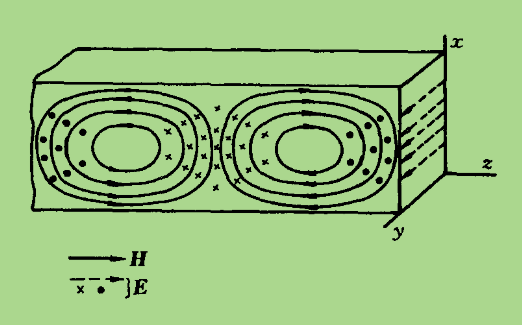
\includegraphics[width=6cm]{figure4-3.png}
       \caption{$TE_{10}$波的电磁场}
   \end{minipage}
   \begin{minipage}[t]{0.48 \textwidth}
       \centering
       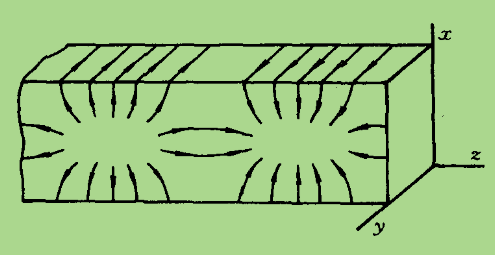
\includegraphics[width=6cm]{figure4-4.png}
       \caption{$TE_{10}$波的管壁电流分布}
   \end{minipage}
   \label{figure4.3&4.4}
   \end{figure}

   可以看出,在$TE_{10}$波情形,波导窄边上没有纵向电流,电流是横过窄边的。印在在波导窄边上任何纵向裂缝都对其的传播有较大的扰动,并导致由裂缝向外辐射电磁波,但横向裂缝却不会影响电磁波在管内的传播。在波导宽边中线处,横向电流为零,因此,开在波导宽边中部的纵向裂缝不会影响到其传播。

   \section{电磁波的辐射}
   \subsection{电磁场的矢势和标势}
   只考虑真空中的电磁场,麦克斯韦方程组为
   \begin{equation}
   \begin{array}{l}{\nabla \times \vec{E}=-\frac{\partial \vec{B}}{\partial t}} \\ {\nabla \times H=\frac{\partial \vec{D}}{\partial t}+\vec{J}} \\ {\nabla \cdot \vec{D}=\rho} \\ {\nabla \cdot \vec{B}=0} \\ {\left(\vec{D}=\varepsilon_{0} \vec{E}, \vec{B}=\mu_{0} \vec{H}\right)}\end{array}
   \end{equation}

   在恒定场中,由$\vec{B}$的无源性引入矢势$\vec{A}$,使
   \begin{equation}
       \vec{B} = \nabla \times \vec{A}
   \end{equation}

\noindent 在一般情况下,$\vec{B}$保持无源性,所以这个关系是普遍成立的。物理意义是:在任何一个时刻,$\vec{A}$沿任一闭合回路的线积分等于该时刻通过回路内的磁通量。

   在变化电磁场下,电场的特性与静电场不同,因为会受到变化磁场的激发,这时电场是有旋的。可以改写为
   \begin{equation}
       \nabla \times \left(\vec{E} + \frac{\partial \vec{A}}{\partial t}\right) = 0
   \end{equation}

\noindent 所以可以用一个标势描述
\begin{equation}
    \vec{E} + \frac{\partial \vec{A}}{\partial t} = - \nabla \cdot \varphi
\end{equation}

\noindent 因此,在一般情况下电场的表示式为
\begin{equation}
    \vec{E} = - \nabla \varphi - \frac{\partial \vec{A}}{\partial t}
\end{equation}

    现在的电场不再是保守力场,一般不存在势能的概念,标势$\varphi$失去作为电场中势能的意义。因此,在高频系统中,电压的概念失去确切的意义。在变化场中,磁场和电场是相互作用着的整体,必须把矢势和标势作为一个整体来描述电磁场。

    \subsubsection{规范变换和规范不变性}
    矢势和标势对电磁场的描述不是唯一的,设$\psi$为任意\textbf{时空函数},作变换
    \begin{equation}
        \begin{aligned}
            \vec{A} \to \vec{A}^{\prime} &= \vec{A} + \nabla \psi \\
            \varphi \to \varphi^{\prime} = \varphi - \frac{\partial \psi}{\partial t} 
        \end{aligned}\label{equ5.1}
    \end{equation}

\noindent 有
\begin{equation}
\begin{array}{c}{\nabla \times \vec{A}^{\prime}=\nabla \times \vec{A}=\vec{B}} \\ {-\nabla \varphi^{\prime}-\frac{\partial \vec{A}^{\prime}}{\partial t}=-\nabla \varphi-\frac{\partial \vec{A}}{\partial t}=\vec{E}}\end{array}
\end{equation}

\noindent 变换\autoref{equ5.1}称为势的规范变换。每一组$(\vec{A},\varphi)$称为一种规范。在经典力学中,由于标势电磁场客观属性的可观测的物理量为$\vec{E}$和$\vec{B}$,而不同规范又对应着同一的$\vec{E}$和$\vec{B}$,因此,如果用势来描述电磁场,客观规律应该和势的特殊的规范选择无关。当势作规范变换时,所有物理量和物理规律都应该保持不变,这种不变性称为\textbf{规范不变性}。

    在量子力学中,电场和磁场不能完全描述电磁场的所有物理效应。在A-B效应中,在飞单连通区域内绕闭合路径一周的电子波函数相位差,就由回路积分
    \begin{equation}
        \oint_C \vec{A} \cdot \mathop{}\!\mathrm{d} \vec{l}
    \end{equation}

\noindent 描述。但是此回路积分仍然是规范不变的,因为对时空函数的梯度求环路积分等于对该函数求环路积分,得到的是零。因此,即使在量子力学中,所有可观测的物理量仍然保持规范不变性。

    可以选择任意的规范,应用最广的是一下两种规范条件:
    \paragraph{库伦规范}
    辅助条件为
    \begin{equation}
        \nabla \cdot \vec{A} = 0
    \end{equation}

\noindent 在这规范中$\vec{A}$为无源场,因而电场表达式为
\begin{equation}
    \vec{E} = - \nabla \varphi - \frac{\partial \vec{A}}{\partial t}
\end{equation}

\noindent 中第二项是无源场(横场),二第一项为无旋场(纵场)。这个规范的特点是电场的纵场部分和横场部分恰好由标势和矢势分别描述。

    \paragraph{洛伦兹规范}
    辅助条件为
    \begin{equation}
        \nabla \cdot \vec{A} + \frac{1}{c^2} \frac{\partial \varphi}{\partial t} = 0
    \end{equation}

\noindent 采用这种规范时,势的基本方程化为特别简单的对称形式,其物理意义也特别明显。

    \subsubsection{达朗贝尔方程}
    利用麦克斯韦方程组推导$\vec{A}$和$\varphi$所满足的基本方程,再分别代入库伦约束和洛伦兹约束得到两种约束下电场、磁场和矢势、标势之间的关系。在洛伦兹约束下得到的这个关系便是\textbf{达朗贝尔方程}。

    现在利用麦克斯韦方程组推导基本方程
    \begin{equation}
        \left \{ \begin{aligned}
            &\nabla \times (\nabla \times \vec{A}) = \mu_0 \vec{J} - \mu_0 \varepsilon_0 \frac{\partial}{\partial t} \nabla \varphi - \mu_0 \varepsilon_0 \frac{\partial^2 \vec{A}}{\partial t^2} \\
            &-\nabla^2 \varphi - \frac{\partial}{\partial t} \nabla \cdot \vec{A} = \frac{\rho}{\varepsilon_0}
        \end{aligned} \right.
    \end{equation}

\noindent 这是适用于一般规范的方程组。

    采用库伦约束
    \begin{equation}
        \left \{ \begin{aligned}
            &\nabla^2 \vec{A} - \frac{1}{c^2 \frac{\partial \vec{A}}{\partial t^2}} - \frac{1}{c^2} \frac{\partial}{\partial t} \nabla \varphi = - \mu_0 \vec{J}\\
            &\nabla^2 \varphi = - \frac{\rho}{\varepsilon_0}
        \end{aligned} \right.
    \end{equation}

\noindent 这种规范的特点是标势所满足的方程与静电场情形相同,其解是库仑势。

    若采用洛伦兹规范,得到
    \begin{equation}
        \left \{ \begin{aligned}
            &\nabla^2 \vec{A} - \frac{1}{c^2} \frac{\partial^2 \vec{A}}{\partial t^2} = - \mu_0 \vec{J}
            & \nabla^2 \varphi - \frac{1}{c^2} \frac{\partial^2 \varphi}{\partial t^2} = -\frac{\rho}{\varepsilon_0}
        \end{aligned} \right.\label{equ5.2}
    \end{equation}

\noindent 用这种规范时,标势和矢势具有相同形式,其意义也非常明显。\autoref{equ5.2}被称为\textbf{达朗贝尔方程},它是非齐次的波动方程,其自由项为电流密度和电荷密度。可以看到,电荷产生标势波动,电流产生矢势波动。离开电荷电流分布区域后,矢势和标势都以波动形式在空间中传播,由它们导出的电磁场也已波动形式在空间中传播。当然电磁场的波动性质是和规范无关的。

    \subsection{推迟势}
    利用达朗贝尔方程,先看标势
    \begin{equation}
        \nabla^{2} \varphi-\frac{1}{c^{2}} \frac{\partial^{2} \varphi}{\partial t^{2}}=-\frac{\rho}{\varepsilon_{0}}
        \end{equation}
    
\noindent 式中$\rho = \rho(\vec{x},t)$ 是空间中的电荷密度。该式是线性方程,反应电磁场的叠加性。由于场的叠加性,可以先考虑某一体元内的变化电荷所激发的势,然后对电荷分布区域积分,即得总的标势。

    不妨设原点处有一假想变化电荷$Q(t)$,其电荷密度为$\rho(\vec{x},t) = Q(t) \delta(\vec{x})$,这时电荷辐射的势的达朗贝尔方程为
    \begin{equation}
        \nabla^{2} \varphi-\frac{1}{c^{2}} \frac{\partial^{2} \varphi}{\partial t^{2}}=-\frac{1}{\varepsilon_{0}} Q(t) \delta(x)\label{equ5.3}
        \end{equation}

\noindent 由球对称性,可知标势不依赖于角变量,所以将\autoref{equ5.3}用球坐标表示,先不考虑原点,并进行如下代换
\begin{equation}
    \varphi(r,t) = \frac{u(r,t)}{r}
\end{equation}

\noindent 可以得到
\begin{equation}
    \frac{\partial^2 u}{\partial r^2} - \frac{1}{c^2} \frac{\partial^2 u}{\partial t^2} = 0
\end{equation}

\noindent 这方程是一维空间下的波动方程,在全空间下可以得到通解
\begin{equation}
    u(r,t) = f(t-\frac{r}{c}) + g(t+\frac{r}{c})
\end{equation}

\noindent 这解得第一项代表向外发射的球面波,第二项代表向内收敛的球面波。对于辐射问题,电磁场是由原点处的电荷发出的,它必然是向外发射的波,因此在辐射问题中应取$g=0$,而函数$f$的形式应由原点处的电荷变化形式决定。利用经典情形下的电势推想\autoref{equ5.3}的解为
\begin{equation}
    \varphi(r,t) = \frac{Q(t-\frac{r}{c})}{4 \pi \varepsilon_0 r} \label{equ5.4}
\end{equation}

    下面来证明这确实是\autoref{equ5.3}的解。当$r \neq 0$时,可以验证确实满足\autoref{equ5.3}。当$r = 0$时,这是一个奇点,猜测具有$\delta$函数形式的奇异性。对此作一半径为$\eta$的小球包围原点,在小球内进行积分,
    \begin{equation}
        \int_{0}^{\eta} 4 \pi r^{2} \mathop{}\!\mathrm{d}  r\left(\nabla^{2}-\frac{1}{c^{2}} \frac{\partial^{2}}{\partial t^{2}}\right) \frac{Q\left(t-\frac{r}{c}\right)}{4 \pi \varepsilon_{0} r}
        \end{equation}

\noindent 当$\eta \to 0$时,积分的第二项$\sim \eta^2$而趋于零,而在第一项中,约去$4 \pi $得到
\begin{equation}
    \int_{0}^{\eta} r^2 \mathop{}\!\mathrm{d} r \frac{1}{r^2} \frac{\partial}{\partial r}\left(r^2 \frac{\partial}{\partial r} \frac{Q(t-\frac{r}{c})}{\varepsilon_0 r}\right)
\end{equation}

\noindent 化简得到
\begin{equation}
    \int_{0}^{\eta} \frac{\partial}{\partial r}\left(r^2 \frac{\partial}{\partial r}\right) \mathop{}\!\mathrm{d} r
\end{equation}

\noindent 由此去掉积分号得到
\begin{equation}
    \left.r^2 \frac{\partial}{\partial r} \frac{Q(t-\frac{r}{c})}{\varepsilon_0 r}\right|_0^{\eta}
\end{equation}

\noindent 计算后发现有对$Q$求导的那一项$\sim r$,所以无论怎样在$\eta \to 0$时都可以认为结果为0,这样就可以得到结果为$-\frac{Q}{\varepsilon_0}$.

    综合$r=0$和$r \neq 0$的情况,可以证明\autoref{equ5.4}确实为\autoref{equ5.3}的解。 

    如果电荷不在原点而是在$x^{\prime}$点上,则令r为其到场点的距离,有
    \begin{equation}
        \varphi(x, t)=\frac{Q\left(x-x^{\prime}, t-\frac{r}{c}\right)}{4 \pi \varepsilon_{0} r}
        \end{equation}

\noindent 由于场的叠加性可以得到一般变化电荷分布$\rho(x^{\prime},t)$所激发的标势,以及根据达朗贝尔方程中矢势所满足的方程形式与标势一致这一特点可以推出矢势的表达式,整理如下
\begin{equation}
    \begin{aligned}
        \varphi(\vec{x}, t)&=\int \frac{\rho\left(\vec{x}^{\prime}, t-\frac{r}{c}\right)}{4 \pi \varepsilon_{0} r} d V^{\prime} \\
        \vec{A}(\vec{x}, t)&=\frac{\mu_{0}}{4 \pi} \int \frac{\vec{J}\left(\vec{x}^{\prime}, t-\frac{r}{c}\right)}{r} d V^{\prime}
    \end{aligned}\label{equ5.5}
\end{equation}

\noindent 可以验证\autoref{equ5.5}满足洛伦兹条件,理论存在自洽性。

    由\autoref{equ5.5}可以看出,在$t$时刻的势并不是在该时刻的电荷和电流产生的,而是在较早时刻$t - \frac{r}{c}$的电荷和电流产生的,所以被称为\textbf{推迟势}。对此也可以从电磁场的传播速度来解释,即电磁场具有有限的传播速度,不是超距作用,传播速度为光速$c$.

    \subsection{电偶极辐射}
    \subsubsection{计算辐射场的一般公式}
    当交变电流分布给定时,利用推迟势公式可以求得辐射场。考虑一定频率的交变电流
    \begin{equation}
        \vec{J}(\vec{x}^{\prime},t) = \vec{J}(\vec{x}^{\prime})e^{-i \omega t}
    \end{equation}

    代入\autoref{equ5.5}第一式可以得到
    \begin{equation}
        \vec{A} (x,t) = \frac{\mu_0}{4 \pi} \int \frac{\vec{J}(\vec{x}^{\prime})e^{i(kr-\omega t)}}{r} \mathop{}\!\mathrm{d} V^{\prime}
    \end{equation}

\noindent 式中$k = \frac{\omega}{c}$为波数。分离位移依赖项和时间依赖项,得到
\begin{equation}
    \vec{A}(\vec{x},t) = \vec{A}(\vec{x}) e^{-i \omega t} 
\end{equation}

\noindent 其中
\begin{equation}
    \vec{A}(\vec{x})=\frac{\mu_{0}}{4 \pi} \int \frac{\vec{J}\left(\vec{x}^{\prime}\right) \mathrm{e}^{\mathrm{i} k r}}{r} \mathrm{d} V^{\prime}\label{equ5.16}
\end{equation}

\noindent $e^{i k r}$是推迟作用因子,它标势电磁波传至场点有相位滞后$kr$.

    电荷密度$\rho$与电流密度$\vec{J}$由电荷守恒定律相联系,在一定频率的交变电流情形有
    \begin{equation}
        i \omega \rho = \nabla \cdot \vec{J}
    \end{equation}

\noindent 因此,只要电流密度$\vec{J}$给定,电荷密度$\rho$便可以求出,由此便可以定出标势。通过电流密度可以得到矢势,由此可以求出磁场,然后利用磁场求出电场
\begin{equation}
    \vec{E} = \frac{ic}{k} \nabla \times \vec{B}
\end{equation}

    \subsubsection{矢势的展开式}
    从$\vec{A}(x,t)$方程中有三个线度:电荷分布区域$l$,波长$\lambda = \frac{2 \pi}{k}$和电荷到场点的距离$r$. 我们只考虑小区域内的电流产生的辐射,即线度远小于波长以及观察距离
    \begin{equation}
        l \ll \lambda, \quad l \ll r \label{equ5.6}
    \end{equation}

\noindent 至于$r$和$\lambda$的关系,可以区别三种情况
\begin{itemize}
    \item 近区 \quad $r \ll \lambda$
    \item 感应区 \quad $r \sim \lambda$
    \item 远区 \quad $r \gg \lambda$
\end{itemize}

    三个区域场的特点不同:在近区,推迟因子趋向于1,因而场保持恒定场的主要特点,即电场具有静电场的纵向形式,磁场也和恒定场类似;在远区内,电磁场变为横向的辐射场;感应场是一个过度区域。实际上,通常是在离发射系统远处接受电磁波的,对这类问题需要计算远场,由远场可定出辐射功率和角分布。但是,如果要研究场对电荷系统的反作用(辐射阻抗)以及几个靠近的发射系统之间的相互影响时,必须计算近场和感应场。我们下面主要讨论远区的场。

    选择坐标原点在电荷分布区域内,则$|x^{\prime}|$的数量级为$l$. 以$R$表示由原点到场点的距离,$r$为由源点$\vec{x}^{\prime}$到$\vec{x}$的距离,有
    \begin{equation}
        r \approx R - \vec{n} \cdot \vec{x}^{\prime}
    \end{equation}

\noindent 其中,$\vec{n}$为沿$\vec{R}$方向的单位矢量。根据\autoref{equ5.6},可以对小参数$\frac{x^{\prime}}{R}$和$\frac{x^{\prime}}{\lambda}$展开。在计算远场时,只保留$\frac{1}{R}$的最低次项,对于
\begin{equation}
    \vec{A}(x)=\frac{\mu_{0}}{4 \pi} \int \frac{\vec{J}\left(\vec{x}^{\prime}\right) \mathrm{e}^{i k\left(\vec{R}-\vec{n} \cdot \vec{x}^{\prime}\right)}}{\vec{R}-\vec{n} \cdot \vec{x}^{\prime}} \mathop{}\!\mathrm{d}  V^{\prime}
\end{equation}

\noindent 由于只保留$\frac{1}{R}$的最低此项,分母中可略去$- \vec{n} \cdot \vec{x}^{\prime}$项,但是相因子中的不可略去,因为这项涉及到的是小参数$\frac{x^{\prime}}{\lambda}$,但相位差这样的一项一般是不可忽略的,所以在相因子展开式保留与之相关的各级项,从而得到
\begin{equation}
    \vec{A}(\vec{x})=\frac{\mu_{0}}{4 \pi} \int \frac{\vec{J}(\vec{x}) e^{i k(\vec{r}-\vec{n} \cdot \vec{x})}}{R-\vec{n} \cdot \vec{x}} \mathop{}\!\mathrm{d} V^{\prime} = \frac{\mu_0 e^{ikR}}{4 \pi R} \int \vec{J}^{\prime} (1-ik\vec{n} \cdot \vec{x}^{\prime} + \cdots) \dif V^{\prime} \label{equ5.9}
\end{equation}

\noindent 展开式中各项对应于各级电磁多级辐射。

    \subsubsection{偶级辐射}
    考虑展开式的第一项
    \begin{equation}
        \vec{A}(\vec{x})=\frac{\mu_{0} e^{i k R}}{4 \pi R} \int \vec{J}(\vec{x}) \mathop{}\!\mathrm{d} V
    \end{equation}

    对于电流密度体积分,由于电流是由运动带电粒子组成的,可以得到
    \begin{equation}
        \int \vec{J}(\vec{x}^{\prime}) \mathop{}\!\mathrm{d} V^{\prime} = \sum e \vec{v}
    \end{equation}

\noindent 又由于
\begin{equation}
    \sum e \vec{v} = \frac{\mathop{}\!\mathrm{d} }{\mathop{}\!\mathrm{d}  t} \sum e \vec{x} = \frac{\mathop{}\!\mathrm{d} \vec{p}}{\mathop{}\!\mathrm{d} t} =\vec{\dot{p}}
\end{equation}

\noindent 所以
\begin{equation}
    \int \vec{J}(\vec{x}^{\prime}) \mathop{}\!\mathrm{d} V^{\prime} = \vec{\dot{p}}\label{equ5.7}
\end{equation}

\noindent 其中,$\vec{p}$是点和系统的电偶极矩。

所以第一项代表振荡电偶极矩产生的辐射
\begin{equation}
    \vec{A}(\vec{x}) = \frac{\mu_0 e^{i k R}}{4 \pi R} \vec{\dot{p}}
\end{equation}

    在计算电磁场时,由于我们只保留$\frac{1}{R}$的最低此项,所以作用结果相当于代换
    .\begin{equation}
        \begin{aligned}
            \nabla & \to i k \vec{n} \\
            \frac{\partial}{\partial t} & \to - i \omega
        \end{aligned}
    \end{equation}

因此 
\begin{equation}
\left\{\begin{aligned}\vec{B}&=\nabla \times \vec{A}=\frac{i \mu_{0} k}{4 \pi R} e^{i k R} \vec{n} \times \vec{\dot{p}}=\frac{1}{4 \pi \varepsilon_0 c^{3} R} e^{i k R} \vec{\ddot{p}} \times \vec{n} \\ \vec{E}&=\frac{i c}{k} \nabla \times \vec{B}=c \vec{B} \times \vec{n}=\frac{e^{i k 2}}{4 \pi \varepsilon_0 c^{2} R}(\vec{\ddot{p}} \times \vec{n}) \times \vec{n}\end{aligned}\right. \label{equ5.14}
\end{equation}

    若取球坐标,原点在电荷分布区,并以$\vec{p}$方向为极轴,则可以得到
    \begin{equation}
    \left\{\begin{aligned}\vec{B}&=\frac{1}{4 \pi \varepsilon_{0} c^{3} R}|\vec{\ddot{p}}| e^{i k R} \sin \theta \vec{e}_{\phi} \\ \vec{E}&=\frac{1}{4 \pi \varepsilon_0 c^{2} R}|\vec{\ddot{p}}| e^{i k R} \sin \vec{\theta} \vec{e}_{\theta}\end{aligned}\right.
    \end{equation}

\noindent 如\autoref{figure5.1}可以看出,磁感线是围绕极轴的圆周,$\vec{B}$总是横向的。电场线是经面上的闭合曲线,\\如\autoref{figure5.2}所示。由于在空间中$\nabla \cdot \vec{E} = 0$,电场线必须闭合,因此电场不可能完全横向,这里横向是因为约去了$\frac{1}{R}$的高次项。因此
\begin{figure}[htbp]
   \centering
   \begin{minipage}[t]{0.48 \textwidth}
       \centering
       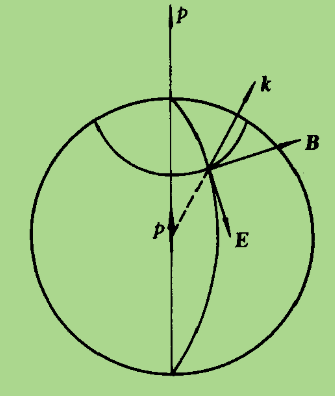
\includegraphics[width=6cm]{figure5-1.png}
       \caption{电磁场方向情况}
   \end{minipage}
   \label{figure5.1}
   \begin{minipage}[t]{0.48 \textwidth}
       \centering
       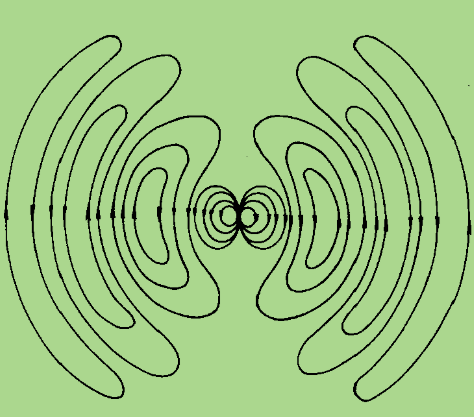
\includegraphics[width=6cm]{figure5-2.png}
       \caption{电磁场是经面上的闭合曲线}
   \end{minipage}
   \label{figure5.2}
   \end{figure}

   \subsubsection{辐射能流,角分布和辐射功率}
   在辐射问题的实际应用中,最主要的问题是计算辐射功率和辐射的方向性,这些都可以由平均能流密度求出。电偶极辐射的平均能流密度为
   \begin{equation}
       \begin{aligned}
           \overline{\vec{S}} &=\frac{1}{2} (\vec{E}^* \times \vec{H}) = \frac{c}{2 \mu_0} \operatorname{Re}\left[(\vec{B}^* \times \vec{n}) \times \vec{B}\right] \\
           &= \frac{c}{2 \mu_0} |\vec{B}|^2 \vec{n} = \frac{|\ddot{\vec{p}}|^2}{32 \pi^2 \varepsilon_0 c^3 R^2} \sin^2 \theta \vec{n}
       \end{aligned}
   \end{equation}

\noindent 可见,电偶极辐射具有方向性,关系为$\sin^2 \theta$,在赤道面上辐射最强,在轴线上没有辐射。将$\overline{\vec{S}}$对球面积分即得总辐射功率P:
\begin{equation}
    \begin{aligned}
        P &= \oint |\overline{S}| R^2 \dif \Omega \\ 
          &= \frac{|\ddot{\vec{p}}|^2}{32 \pi^2 \varepsilon_0 c^3} \oint \sin^2 \theta \dif \Omega \\ 
          &= \frac{1}{4 \pi \varepsilon_0}\frac{|\ddot{\vec{p}}|^2}{3c^3}
    \end{aligned}\label{equ5.8}
\end{equation}

\noindent 由此看出,若保持电偶极矩振幅不变,则辐射正比于频率的四次方。频率变高时,辐射功率迅速增大。

    \subsubsection{短天线的辐射}
    当直线天线的长度l远小于波长时,它的辐射就是电偶极辐射。\autoref{figure5.3}表示中心馈电的长度为l的天线。可以发现,在天线两半段上,电流方向相同,在天线两端电流为零。若天线长度$l \ll \lambda$,则沿天线上的电流分布近似为线性形式。
    \begin{figure}[htb]
        \centering
        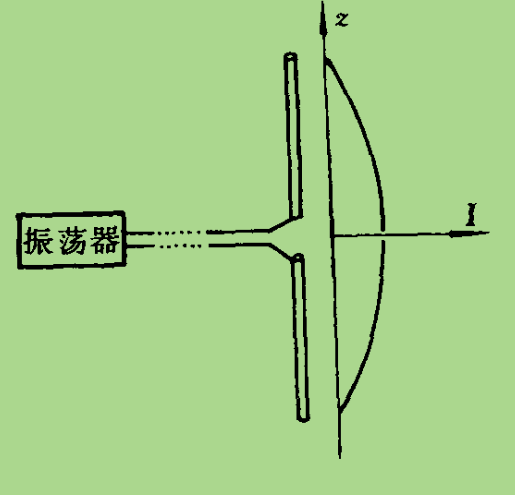
\includegraphics[width=8cm]{figure5-3.png}
        \caption{短天线的电流分布}
        \label{figure5.3}
    \end{figure}

    \begin{equation}
        I(z) = I_0 \left(1- \frac{2}{l} |z|\right)
    \end{equation}

\noindent 由于\autoref{equ5.7},电偶极矩变化率为
\begin{equation}
    \dot{\vec{p}} = \int_{-l/2}^{l/2} \vec{I}(z) \dif z = \frac{1}{2} I_0 l
\end{equation}

\noindent 由\autoref{equ5.8}得到短天线的辐射功率
\begin{equation}
    P = \frac{\mu_0 I_0^2 \omega^2 l^2}{48 \pi c} = \frac{\pi}{12} \sqrt{\frac{\mu_0}{\varepsilon_0}}I_0^2 \left(\frac{l}{\lambda}\right)^2
\end{equation}

\noindent 这式子适用于$l \ll \lambda$的情形。由此式看出,若保持天线电流$I_0$不变,则短天线的辐射功率正比于$\left(\frac{l}{\lambda}\right)^2$.

    由于电磁能量不断向外辐射,电源需要供给一定的功率来维持辐射。由于辐射功率正比于$I_0^2$,辐射功率相当于一个等效电阻上的损耗功率,这个等效电阻称为辐射电阻$R_r$. 由于$I_0$是电流的最大值,类比交流电下的辐射公式(相比直流电,低频交流电用电流最大值代替电流,但形式上需要乘上一个$\frac{1}{2}$)可以得到等效电阻
    \begin{equation}
        R_r = \frac{\pi}{6} \sqrt{\frac{\mu_0}{\varepsilon_0}} \left(\frac{l}{\lambda}\right)^2
    \end{equation}

    \subsection{磁偶级辐射和电四级辐射}
    \subsubsection{高频电流分布的磁偶极矩和电四极矩}
    考虑辐射矢势展开式\autoref{equ5.9}的第二式
    \begin{equation}
        \vec{A}(x) = \frac{-i k \mu_0 e^{ikR}}{4 \pi R} \int \vec{J} (\vec{n} \cdot x^{\prime}) \dif V^{\prime}\label{equ5.10}
    \end{equation}

\noindent 当电流分布的电偶极矩变为零时,这项变为主要项,这代表的是磁偶极矩和电四极矩。

    在交变情形下,由于电流一般不闭合,电流分布往往和电荷分布相联系,由电荷守恒定律得到
    \begin{equation}
        i \omega \rho = \nabla \cdot \vec{J}
    \end{equation}

    现在把\autoref{equ5.10}中的积分分离为磁矩的贡献和电四极矩的贡献,先把被积函数写作
    \begin{equation}
        \vec{J}^{\prime}(\vec{n} \cdot \vec{x}^{\prime}) = \vec{n} \cdot \vec{x}^{\prime} \vec{J}^{\prime}
    \end{equation}

\noindent $\vec{x}^{\prime} \vec{J}^{\prime}$ 是一个张量,可以分解为对称部分和反对称部分
\begin{equation}
    \vec{x}^{\prime} \vec{J}^{\prime} = \frac{1}{2} (\vec{x}^{\prime} \vec{J}^{\prime} + \vec{J}^{\prime} \vec{x}^{\prime}) + \frac{1}{2} (\vec{x}^{\prime} \vec{J}^{\prime} - \vec{J}^{\prime} \vec{x}^{\prime})
\end{equation}

\noindent 代入积分式中。先看第二项,由于
\begin{equation}
    \left(\vec{n} \cdot \vec{x}^{\prime}\right) \vec{J}^{\prime}-\left(\vec{n} \cdot \vec{J}^{\prime}\right) \vec{x}^{\prime}=-\vec{n} \times\left(\vec{x}^{\prime} \times \vec{J}^{\prime}\right)
\end{equation}

\noindent 因而第二式为
\begin{equation}
    - \vec{n} \times \int \frac{1}{2} \vec{x}^{\prime} \times \vec{J}^{\prime} \dif V^{\prime} = - \vec{n} \times \vec{m} \label{equ5.11}
\end{equation}

\noindent 其中$\vec{m}$是磁偶极矩,因而这一项是偶级辐射。

    再看第一项,可以把它写作对所有带电粒子求和
    \begin{equation}
    \begin{aligned} & \frac{1}{2} \int\left[\left(\vec{n} \cdot \vec{x}^{\prime}\right) \vec{J}^{\prime}+\left(\vec{n} \cdot \vec{J}^{\prime}\right) \vec{x}^{\prime}\right] \mathrm{d} V \\=& \frac{1}{2} \sum e\left[\left(\vec{n} \cdot \vec{x}^{\prime}\right) \vec{v}^{\prime}+\left(\vec{n} \cdot \vec{v}^{\prime}\right) \vec{x}^{\prime}\right] \end{aligned}
    \end{equation}

\noindent 将速度表示为对时间的导数,可将上式改写成
\begin{equation}
    \frac{1}{6} \vec{n} \cdot \frac{\dif }{\dif t} \mathbf{\mathscr{D}}  = \frac{1}{6} \vec{n} \cdot \mathbf{\mathscr{D}} \label{equ5.12}
\end{equation}

\noindent 式中 
\begin{equation}
    \mathbf{\mathscr{D}} = \sum 3e \vec{x}^{\prime} \vec{x}^{\prime}
\end{equation}

\noindent 是体系电四极矩,是一个张量。

    将\autoref{equ5.11}和\autoref{equ5.12}代入\autoref{equ5.10}得到
    \begin{equation}
        \vec{A} = - \frac{i k \mu_0 e^{ik R}}{4 \pi R} \left[- \vec{n} \times \vec{m} + \frac{1}{6} \vec{n} \cdot \mathbf{\mathscr{D}}\right]\label{equ5.13}
    \end{equation}
    
\noindent 第一项是磁偶极矩辐射式,第二项是电偶极矩辐射式。

    \subsubsection{磁偶级辐射}
    对于\autoref{equ5.13}第一项,由此得到磁偶极矩的辐射电磁场
    \begin{equation}
    \begin{aligned} \vec{B} &=\nabla \times \vec{A}=\mathrm{i} k \vec{n} \times \vec{A} \\ &=k^{2} \frac{\mu_{0} \mathrm{e}^{\mathrm{i} k R}}{4 \pi R}(\vec{n} \times \vec{m}) \times \vec{n} \\ &=\frac{\mu_{0} \mathrm{e}^{\mathrm{i} k R}}{4 \pi c^{2} R}(\ddot{\vec{m}} \times \vec{n}) \times \vec{n} \\ \vec{E} &=c \vec{B} \times \vec{n}=-\frac{\mu_{0} \mathrm{e}^{\mathrm{i} k R}}{4 \pi c R}(\ddot{\vec{m}} \times \vec{n}) \end{aligned}\label{equ5.15}
    \end{equation}

\noindent 将\autoref{equ5.14}和\autoref{equ5.15}进行比较,可见通过电偶极辐射场作如下代换
\begin{equation}
    \begin{aligned}
        \vec{p} &\to \frac{\vec{m}}{c} \\
        \vec{E} & \to c \vec{B} \\ 
        c\vec{B} &= \to - \vec{E}
    \end{aligned}
\end{equation}

\noindent 即得磁偶级辐射场。这代换反映麦克斯韦方程组的电磁对称性。在自由空间中,麦氏方程组对变换$\vec{E} \to c \vec{B},c \vec{B} \to - \vec{E}$是对称的,若其中一个是解,另一个也定然是解。

    磁偶级辐射的能流密度和总辐射功率为
    \begin{equation}
        \begin{aligned}
            \vec{S} &= \frac{\mu_0 \omega^4 |\vec{m}|^2}{32 \pi^2 c^3 R^2} \sin^2 \theta \vec{n} \\
            P &= \frac{\mu_0 \omega^4 |\vec{m}|^2}{12 \pi c^3}
        \end{aligned}
    \end{equation}

    \subsubsection{电四级辐射}
    现在计算\autoref{equ5.13}的第二项,这对应着电四极矩辐射的电磁场。先定义矢量
    \begin{equation}
        \vec{\mathscr{D}}(\vec{n}) = \vec{n} \cdot \mathbf{\mathscr{D}}
    \end{equation}

\noindent 则矢势表达式为
\begin{equation}
    \vec{A}(x)=-\frac{i k \mu_{0} e^{i k R}}{24 \pi R} \vec{\mathscr{D}}=\frac{\mathrm{e}^{\mathrm{i} k R}}{24 \pi \varepsilon_{0} c^{3} R} \vec{\mathscr{D}}
\end{equation}

\noindent 这里利用了$\frac{\partial}{\partial t} = - i \omega  = - i k /c$,这个式子能够成立是由于我们现在考虑的都是单频电磁波的情况,在这种情况下时间依赖项都是$e^{-i \omega t}$. 由此得到辐射区电磁场为\footnote{注意$\tilde{\mathscr{D}}$代表对时间的三阶导,因为我实在不知在LaTeX中如何打出三个在上面的点,就这样代替了。后面的若出现这个符号大概率也是同样的原因}
\begin{equation}
    \begin{aligned}
        \vec{B} &= ik \vec{n} \times \vec{A} = \frac{e^ikR}{24 \pi \varepsilon_0 c^4 R}
        \tilde{\vec{\mathscr{D}}} \times \vec{n} \\
        \vec{E} &=c \vec{B} \times \vec{n} = \frac{e^{ikR}}{24 \pi \varepsilon_0 c^3 R} (\tilde{\vec{\mathscr{D}}} \times \vec{n}) \times \vec{n}
    \end{aligned}
\end{equation}

\noindent 由上式知道对电四极矩加上与$\vec{n}$成正比的项并不影响辐射区电磁场,因此和恒定场一样,将电四极矩定义为
\begin{equation}
    \mathbf{\mathscr{D}} = \sum e(3\vec{x}^{\prime} \vec{x}^{\prime}- (r^{\prime})^2 E)
\end{equation}

\noindent 其中$E$是单位矩阵。

    辐射平均能流密度是(直接代入公式就可以得到,故直接给答案)$\overline{\vec{S}} = \frac{1}{4 \pi \varepsilon_0} \frac{1}{288 \pi c^5 R^2} (\tilde{\vec{\mathscr{D}}} \times \vec{n})^2$.

\noindent 设电荷分布区域线度为$l$,可以验证,电四极矩与磁偶极辐射同级,但比电偶极辐射小$(l/\lambda)^2$数量级。

    \subsection{天线辐射}
    \subsubsection{天线上的电流分布}
    当天线线度与波长同数量级时,必须直接使用\autoref{equ5.15}而不能用展开式\autoref{equ5.9}. 取天线沿着z轴方向,电流$\vec{J}$也沿着z轴,因而$\vec{J}$也只有z分量。取洛伦兹条件
    \begin{equation}
        \left \{ \begin{aligned}
            &\nabla \cdot \vec{A} + \frac{1}{c^2} \frac{\partial \varphi}{\partial t} = 0 \\ 
            &E_z = - \frac{\partial \varphi}{\partial z} - \frac{\partial A_z}{\partial t}
        \end{aligned} \right.
    \end{equation}

\noindent 所以 
\begin{equation}
    \frac{1}{c^2} \frac{\partial E_z}{\partial t} = \frac{\partial^2 A_z}{\partial z} - \frac{1}{c^2} \frac{\partial^2 A_z}{\partial t^2}
\end{equation}

    设天线为理想导体,在天线表面,电场切向分量$E_z = 0$,因而在天线表面$A_z$满足一维波动方程 
    \begin{equation}
        \frac{\partial^2 A_z}{\partial t} - \frac{1}{c^2} \frac{\partial^2 A_z}{\partial t^2} = 0
    \end{equation}

\noindent 矢势$\vec{A}$与天线电流的关系式是推迟势公式\autoref{equ5.16}. 我们可以将$\vec{J}(z^{\prime})$作为未知量,然后求解\\
\autoref{equ5.16},边界条件是端点处$\vec{J} = 0$. 所以这就是一个求解积分方程的问题,但很显然,这个问题的一般情况我们是不会的,一想就知道会很困难,所以我们只考虑天线截面很小时的近似情况。当天线很小时,当场点和源点的z坐标靠近时,r变得很小,对\autoref{equ5.16}的积分贡献较大,所以在这情形下,$\vec{A}_z$主要与$z^{\prime} \approx z$的电流有关,因而$\vec{J}(z^{\prime})$应该近似于$\vec{A}(z)$的形状,即也是波动形式。考虑到端点固定,理应是驻波形式。注意这个近似只有在截面很小的时候才成立。

    \subsubsection{半波天线}
    设有中心馈电的直线状天线,天线上的电流近似为驻波形式,两端为波节。设天线总长度为$l$,电流分布为 
    \begin{equation}
        \left \{ \begin{aligned}
            &I_0 \sin k\left(\frac{l}{2} - z\right) \\
            &I_0 \sin k\left(\frac{l}{2} + z\right) 
        \end{aligned} \right.
    \end{equation}

\noindent 若$l = \lambda /2$,上式化为
\begin{equation}
    I(z) = I_0 \cos k z \qquad |z| \le \frac{\lambda}{4}
\end{equation}

    利用矢势公式\autoref{equ5.16},令$\vec{J}^{\vec{x}^{\prime}} \dif V^{\prime}$改为$I \dif \vec{l}$,从而得到 
    \begin{equation}
        A_z(x) = \frac{\mu_0}{4 \pi} \int_{\frac{\lambda}{4}}^{-\frac{\lambda}{4}} \frac{e^{ikr}}{r} I_0 \cos k z \dif z
    \end{equation}

\noindent 计算远场时令
\begin{equation}
    r = R - z \cos \theta 
\end{equation}

\noindent 其中$R$为原点到场点的距离。取$\frac{1}{R}$最低此项时,分母中的r可取代为R,由此得到
\begin{equation}
    A_z(x) = \frac{\mu_0}{4 \pi} \frac{I_0 e^{ikR}}{R} \int_{\frac{\lambda}{4}}^{-\frac{\lambda}{4}} \cos k z e^{-ikz \cos \theta} \dif z
\end{equation}

\noindent 最终得到
\begin{equation}
    \vec{A}(\vec{x})=\frac{\mu_{0} I_{0} e^{i k R}}{2 \pi k R} \frac{\cos \left(\frac{\pi}{2} \cos \theta\right)}{\sin ^{2} \theta} \vec{e}_{z}
\end{equation}

    由此算出辐射区的电磁场以及平均辐射能流密度。辐射角由因子
    \begin{equation}
        \frac{\cos^2 \left(\frac{\pi}{2} \cos \theta\right)}{\sin^2 \theta}
    \end{equation}

\noindent 确定。它与偶级辐射角分布相似,但较集中于$\theta = 90^{\circ}$平面上。

    \subsubsection{天线阵}
    半波天线对于极角$\theta$有一定的方向性,对方位角没有方向性。要得到高度定向的辐射,可以用一系列天线排成天线阵,利用各条天线辐射的干涉效应还获得较强的方向性。

    \subsection{电磁波的衍射}
    在光学中衍射理论的基础是惠更斯原理,这原理假设光波面上每一点可以看作次级光源,它们发射出子波,这些子波叠加后得到向前传播的光波。
    \subsubsection{从电动力学基本原理出发推导惠更斯原理}
    考虑典型的衍射问题\autoref{figure5.4}:设屏幕上有一小孔,电磁波从左边入射,我们要计算通过小孔后在屏幕右边各点上的电磁波场强。这问题严格来说应该作为边值问题求解,但十分复杂,采取近似。
    \begin{figure}[htb]
        \centering
        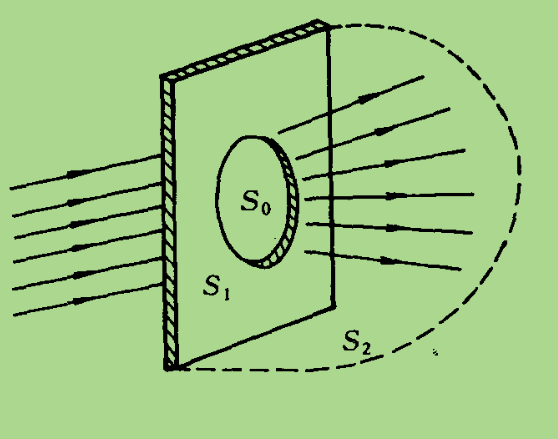
\includegraphics[width=8cm]{figure5-4.png}
        \caption{典型的衍射问题}
        \label{figure5.4}
    \end{figure}

    近似的主要点是假设小孔上和屏幕右侧的场强为已知,由此求出右半空间各点上的场强。这种求解方法实质上是把一个区域的电磁场用其边界的值表示出来。第二个近似的方面在于忽略电磁场中的矢量性,而采用标量场的衍射理论来求解。当衍射角不大的时候这是较好的近似。

    利用基尔霍夫公式
    \begin{equation}
        \nabla^2 \psi + k^2 \psi = 0
    \end{equation}

\noindent 其中$\psi$可以代表电磁场中任一直角分量。

    在忽略电磁场其他分量的影响而独立地把$\psi$看作标量场,并用边界上的$\psi$和$\frac{\partial \psi }{\partial n}$值表示区域内的$\psi$,这种理论便是\textbf{标量衍射理论}。

    同在静电场中情况一样使用格林公式和格林函数。设$G(\vec{x},\vec{x}^{\prime})$是亥姆霍兹方程的格林函数
    \begin{equation}
        (\nabla^2 + k^2)G(\vec{x},\vec{x}^{\prime}) = 4 \pi \delta (\vec{x}- \vec{x}^{\prime})
    \end{equation}

\noindent 对于
\begin{equation}
    \left(\nabla^{2}-\frac{1}{c^{2}} \frac{\partial^{2}}{\partial t^{2}}\right) \frac{Q\left(t-\frac{r}{c}\right)}{4 \pi \varepsilon_{0} r}=-\frac{1}{\varepsilon_{0}} Q(t) \delta(x)
\end{equation}

\noindent 令$Q(t) = 4 \pi \varepsilon_0 e^{-i \omega t}$,可以看出(凑出)具有出射波形式的格林函数为
\begin{equation}
    G(\vec{x},\vec{x}^{\prime}) = \frac{e^{ikr}}{r}
\end{equation}

    将$G$和$\psi$代入格林公式
    \begin{equation}
    \begin{aligned} &\int_{V} \left[\psi\left(\vec{x}^{\prime}\right) \nabla^{\prime 2} G\left(\vec{x}^{\prime}, \vec{x}\right)-G\left(\vec{x}^{\prime}, \vec{x}\right) \nabla^{\prime 2} \psi\left(\vec{x}^{\prime}\right)\right] \dif V^{\prime} \\ &=\oint_{S}\left[\psi\left(\vec{x}^{\prime}\right) \nabla^{\prime} G\left(\vec{x}^{\prime}, \vec{x}\right)-G\left(\vec{x}^{\prime}, \vec{x}\right) \nabla^{\prime} \psi\left(\vec{x}^{\prime}\right)\right] \cdot \dif \vec{S}\end{aligned}
    \end{equation}

\noindent 为方便起见,设$\vec{n}$是指向区域V\red{内}的法线,即$\dif \vec{S}^{\prime} = - \vec{n} \dif S^{\prime}$,由此得到
\begin{equation}
    \begin{aligned}
        \psi(\vec{x}) &= - \frac{1}{4 \pi} \oint_{S} \left[\psi(\vec{x}) \nabla^{\prime} \frac{e^{ikr}}{r} - \frac{e^{ikr}}{r} \nabla^{\prime} \psi(\vec{x}^{\prime})\right] \cdot \dif \vec{S}^{\prime}  \\
        &= - \frac{1}{4 \pi} \oint_S \frac{e^{ikr}}{r} \vec{n} \cdot \left[\nabla^{\prime} \psi +\left(ik-\frac{1}{r}\right) \frac{\vec{r}}{r} \psi\right] \dif S^{\prime}
    \end{aligned}\label{equ5.17}
\end{equation}

    这被称为\textbf{基尔霍夫公式}。这公式把区域V内任一点的场用边界面上的场和场对法向的导数表示出来。可以看出,基尔霍夫公式是惠更斯原理的数学表示,因子$\frac{e^{ikr}}{r}$表示由曲面S上的点$\vec{x}$向V内$\vec{x}$点传播的波,波源的强度由$\vec{x}^{\prime}$点上的$\psi$和$\frac{\partial \psi}{\partial n}$值确定。因此,曲面上每一点可以看作次级光源,区域V内的光波可以看作由曲面所有点上的次级光源发射的子波的叠加。

    但这还不是边值问题的解,因为边界条件尚未确定,当问题完全解出之前,边界条件是不可知的,但也不能任意规定。所以,只有在某些特殊的情况下,当我们可以合理的估计边界条件时,才能应用\autoref{equ5.17}. 衍射问题通常属于这种情况。

    \subsubsection{小孔衍射}
    设无穷大平面中部有一小孔,$V$为屏幕右边空间,其界面$S$分为三个部分
    \begin{itemize}
        \item 小孔表面$S_0$
        \item 屏幕右侧$S_1$
        \item 无穷大半球面$S_2$
    \end{itemize}

\noindent 为了应用基尔霍夫公式,必须对界面上的$\psi$和$\frac{\partial \psi}{\partial n}$值作合理的假定。我们做以下假设
\begin{itemize}
    \item 在孔面$S_0$上,$\psi$和$\frac{\partial \psi}{\partial n}$等于原来入射波的值,即和没有屏幕存在时相同
    \item 屏幕右侧上,$\psi = \frac{\partial \psi}{\partial n} = 0$
\end{itemize}

    当孔半径远大于波长时,大部分场不受扰动(只有小孔边缘附近入射波存在较大的扰动),(1)近似成立;只有小孔边缘处$\psi$和$\frac{\partial \psi}{\partial n}$才可能显著不为零,(2)也可近似成立。

    为了计算$\psi$,还必须知道无穷远半球面$S_2$上的$\psi$值。如\autoref{figure5.5-6}左图,取坐标原点在小孔中心处,以$\vec{x}^{\prime}$表示$S_2$上的一点,$\vec{x}$为区域内距离小孔有限远处任一点。令$R = |\vec{x}|$,$R^{\prime} = |\vec{x}^{\prime}|$,$r = |\vec{x}-\vec{x}^{\prime}|$. 由于在右半空间的波是小孔区出射的波,因此在无穷远处有如下形式
    \begin{equation}
        \psi(\vec{x}^{\prime}) = f(\theta^{\prime},\phi^{\prime}) \frac{e^{ikR^{\prime}}}{ R^{\prime}}
    \end{equation}

\noindent $f(\theta^{\prime},\phi^{\prime})$代表与方向有关的某一函数,在$S_2$上,向内法线为$\vec{n} = - \vec{e}_R^{\prime}$,因而 
\begin{equation}
    \vec{n} \cdot \nabla^{\prime} \psi = - \frac{\partial}{\partial R^{\prime}} \psi(\vec{x}^{\prime}) = -(ik - \frac{1}{R^{\prime}}) \psi 
\end{equation}

\noindent 当$r \to \infty$时,$\vec{r}/r \approx \vec{n}$,$1/r \approx 1/R^{\prime}$,因此在$S_2$上到$O(r^{-2})$有
\begin{equation}
    \vec{n} \cdot \left[\nabla^{\prime} \psi +\left(ik-\frac{1}{r} \right)\frac{\vec{r}}{r}\psi\right] \approx 0
\end{equation}

\noindent 因而\autoref{equ5.17}中对于无穷大半球面的积分趋于零,而只剩下了对孔面的积分
\begin{equation}
    \psi(\vec{x}) = - \frac{1}{4 \pi} \int_{S_0} \frac{e^{ikr}}{r} \vec{n} \cdot \left[\nabla^{\prime} \psi +\left(ik-\frac{1}{r}\right) \frac{\vec{r}}{r}\psi\right] \dif S^{\prime} \label{equ5.18}
\end{equation}

    \begin{figure}[htbp]
       \centering
       \begin{minipage}[t]{0.48 \textwidth}
           \centering
           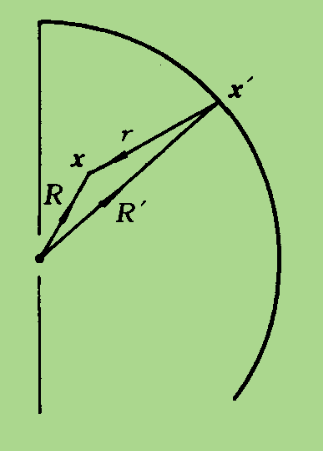
\includegraphics[width=6cm]{figure5-5.png}
           \caption{无穷大半球面的场}
       \end{minipage}
       \begin{minipage}[t]{0.48 \textwidth}
           \centering
           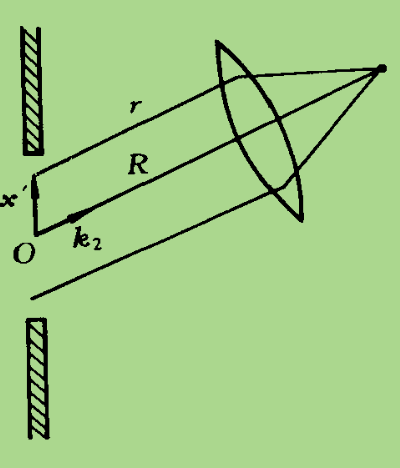
\includegraphics[width=6cm]{figure5-6.png}
           \caption{夫琅禾费衍射}
       \end{minipage}
       \label{figure5.5-6}
       \end{figure}

    由假设(1),设入射波$\psi_i$是平面波,其波矢量为$\vec{k}_1$,
    \begin{equation}
        \psi_i(\vec{x}^{\prime}) = \psi_0 e^{i\vec{k}_1 \cdot \vec{x}^{\prime}}
    \end{equation}

\noindent 其中$\psi_0$为原点处的$\psi$值。用$\psi_i$代入\autoref{equ5.18}中的$\psi$,并有
\begin{equation}
    \nabla^{\prime} \psi(\vec{x}^{\prime}) = i \vec{k}_1 \psi_0 e^{i \vec{k}_1 \cdot \vec{x}^{\prime}}
\end{equation}

    设我们在屏幕右边远处观察向$\vec{k}_2$方向传播的衍射波(实际观察时可用透镜将其聚焦,这种衍射称为\textbf{夫琅禾费衍射})。如\autoref{figure5.5-6}右图,由于$\vec{k}_2$沿着R方向,则$r = R - \frac{\vec{k}_2}{k} \cdot \vec{x}^{\prime}$,$k \frac{\vec{r}}{r} = \vec{k}_2$,在\autoref{equ5.18}略去$\frac{1}{r}$高次项,得到
    \begin{equation}
        \begin{aligned}
            \psi(\vec{x}) &=- \frac{i \psi_0 e^{ikR}}{4 \pi R} \int_{S_0} e^{i(\vec{k}_1 - \vec{k}_2} \cdot \vec{x}^{\prime}(\vec{k}_1 + \vec{k}_2) \cdot \vec{n} \dif S^{\prime} \\
            &=- \frac{i \psi_0 e^{ikR}}{4 \pi R} \int_{S_0} e^{i(\vec{k}_1 - \vec{k}_2} \cdot \vec{x}^{\prime} (\cos \theta_1 + \cos \theta_2) \dif S^{\prime}
        \end{aligned}
    \end{equation}

\noindent 其中,$\theta_1$和$\theta_2$分别是法线、衍射波波矢与$\vec{n}$夹角,而$(\cos \theta_1 + \cos \theta_2)$便是著名的\textbf{倾斜因子}。

    \subsection{电磁场的动量}
    电磁场和带电物质之间有相互作用。场对带电粒子施加作用力,粒子受力后,它的动量发生变化,同时电磁场本身的状态亦发生相应的改变。事实上,电磁波对物体的作用是通过对物体内的带电粒子的受力而使物理受到一定的总力,由于物体受力动量会发生改变,根据动量守恒,这意味着电磁场的动量发生改变,也就是说,电磁场存在动量。下面从电磁场和带电物质的相互作用规律推导出电磁场动量密度表示式。

    \subsubsection{电磁场的动量密度和动量流密度}
    考虑空间某一区域,有一定的电荷分布。区域内的场和电荷之间由于相互作用而发生动量转移;另一方面,区域内的场和区域外的场也通过界面发生动量转移。由于动量守恒,单位时间从区域外通过界面$S$传入区域内的动量应该等于区域内电荷的动量变化率加上区域内电磁场的动量变化率
    \begin{equation}
        \nabla \cdot \vec{P} + \frac{\partial \vec{p}}{\partial t} + \frac{\partial \vec{p}^{\prime}}{\partial t} =0
    \end{equation}

\noindent 其中$\vec{P}$是通过边界的动量,$\vec{p}$和$\vec{p}^{\prime}$是区域内的电荷动量和场的动量。

    电荷受电磁场的作用力由洛伦兹力公式表示。以$\vec{f}$表示作用力密度,得到
    \begin{equation}
        \vec{f} = \rho \vec{E} + \vec{J} \times \vec{B}\label{equ5.22}
    \end{equation}

\noindent 电荷系统受力作用后,它的动量发生变化。由动量守恒定律,电磁场的动量也应该相应地改变。\autoref{equ5.22}左边等于电荷系统的动量密度变化率,因而右边可以化为含有电磁场动量密度变化率和表示场内动量转移的一些量。我们可以用麦克斯韦方程组把\autoref{equ5.22}右边完全用场量表示。考虑
\begin{equation}
    \left \{ \begin{aligned}
        &\rho = \varepsilon_0 \nabla \cdot \vec{E} \\
        &\vec{J} = \frac{1}{\mu_0} \nabla \times \vec{B} - \varepsilon_0 \frac{\partial \vec{E}}{\partial t}
    \end{aligned} \right.
\end{equation}

\noindent 从而得到
\begin{equation}
    \vec{f} = \varepsilon_0 (\nabla \cdot \vec{E}) + \frac{1}{\mu_0}(\nabla \times \vec{B})\times \vec{B} - \varepsilon_0 \frac{\partial \vec{E}}{\partial t} \times \vec{B}
\end{equation}

\noindent 利用磁场无旋性和电场散度关系写成更加对称的形式
\begin{equation}
    \begin{aligned}
        \vec{f} &= \left[\varepsilon_0 (\nabla \cdot \vec{E}) \vec{E} + \frac{1}{\mu_0} (\nabla \cdot \vec{B}) \vec{B} + \frac{1}{\mu_0} (\nabla \times \vec{B}) \times \vec{B} \right.\\
        &+ \left.\varepsilon_0(\nabla \times \vec{E}) \times \vec{E}\right] - \varepsilon_0 \frac{\partial (\vec{E} \times \vec{B})}{\partial t}\label{equ5.19}
    \end{aligned}
\end{equation}

    由于$\vec{f}$等于电荷系统的动量密度改变率(从力的定义可知),因此,若把\autoref{equ5.19}解释为动量守恒定律,则右边最后一项去掉负号意味着动量密度改变率,因此电磁场的动量密度可以定义为
    \begin{equation}
        \vec{g} = \varepsilon_0 \vec{E} \times \vec{B}
    \end{equation}

\noindent \autoref{equ5.19}方括号部分可以表示电磁场内部的动量转移,令
\begin{equation}
    \mathbf{\mathscr{D}} \equiv - \varepsilon_0 \vec{E} \vec{E} - \frac{1}{\mu_0} + \frac{1}{2} \mathbf{I}\left(\varepsilon_0 E^2 + \frac{1}{\mu_0}B^2\right)
\end{equation}

\noindent 从而得到动量守恒定律的微分式
\begin{equation}
    \vec{f} + \frac{\partial \vec{g}}{\partial t} = - \nabla \cdot \mathbf{\mathscr{D}} \label{equ5.20}
\end{equation}

\noindent 注意这个式子中左右两边的结果都是张量,其中张量$\mathbf{\mathscr{D}}$被称为\textbf{电磁场的动量流密度张量},或称为\textbf{电磁场应力张量}。

    若区域为全空间,对\autoref{equ5.20}积分可得
    \begin{equation}
        \int_V \vec{f} \dif V + \frac{\dif}{\dif t} \int_V \vec{g} \dif V = - \oint_S \dif \vec{S} \cdot \mathbf{\mathscr{D}}
    \end{equation}

\noindent 全空间下,表面积分趋于零,由此可以得到
\begin{equation}
    \int \vec{f} \dif V + \frac{\dif }{\dif t} \int \vec{g} \dif V =0 \label{equ5.21}
\end{equation}

\noindent 这就是\textbf{动量守恒定律}。

    电磁场的动量密度和能流密度之间存在如下关系
    \begin{equation}
        \vec{g} = \varepsilon_0 \vec{E} \times \vec{B} = \varepsilon_0 \mu_0 \vec{E} \times \vec{H} = \frac{1}{c^2} \vec{S}\label{equ5.23}
    \end{equation}

\noindent 由于对电磁波有$\vec{S} = c w \vec{n}$,其中$\vec{n}$是传播方向单位矢量,$w$是能量密度,因此
\begin{equation}
    \vec{g} = \frac{w}{c} \vec{n}
\end{equation}

    通过动量流密度张量可以求出通过面元的动量,具体关系如下
    \begin{equation}
        \begin{aligned}
            \Delta p_{1}&=\Delta S_{1} T_{11}+\Delta S_{2} T_{21}+\Delta S_{3} T_{31}\\
            \Delta p_{2}&=\Delta S_{1} T_{12}+\Delta S_{2} T_{22}+\Delta S_{3} T_{32}\\
            \Delta p_{3}&=\Delta S_{1} T_{13}+\Delta S_{2} T_{23}+\Delta S_{3} T_{33}\\
        \end{aligned}
    \end{equation}

\noindent 或写成矢量式
\begin{equation}
    \Delta \vec{p} = \Delta \vec{S} \cdot \mathbf{\mathscr{D}}
\end{equation}

\noindent 因此通过闭合曲面流出的总动量为
\begin{equation}
    \oint \dif \vec{S} \cdot \mathbf{\mathscr{D}}
\end{equation}

\noindent 更进一步,电磁场应力张量的分量$T_{ij}$的意义是通过垂直于$i$轴的单位面积流过的动量$j$分量。

    \subsubsection{辐射压力}
    由于电磁波具有动量,它入射于物体上时会对物体施加一定的压力了,这种压力称为辐射压力。有电磁波动量密度和能量密度关系\autoref{equ5.23}和动量守恒定律\autoref{equ5.21}可以算出辐射压强。注意压强和能量密度是同一量纲。对于平面电磁波入射理想导体被全部反射这个例子,假设入射角为$\theta$,用两种办法东可以算符导体表面所受的辐射压强为
    \begin{equation}
        P = \overline{w} \cos^2 \theta
    \end{equation}

    \section{狭义相对论}
    \subsection{相对论基本原理和洛伦兹变换}
    \subsubsection{相对论基本原理}
    \begin{itemize}
        \item 相对性原理:所有惯性参考系都是等价的。物理规律对于所有惯性参考系都可以表示为相同形式,任何物理现象都无法觉察出所处参考系的任何“绝对运动”。这体现出物理定律对于(惯性)参考系的客观性。
        \item 光速不变原理:真空中的光速相对于任何惯性系沿任一方向恒为c,并与光源运动无关。
    \end{itemize}

    可以用一个简单例子看出光速不变性与旧时空的矛盾性。考虑两个光源,其中一个静止,位于$\sum$惯性系;另一个沿着x轴匀速直线运动,位于$\sum^{\prime}$惯性系。光源发出的光同时到达的地方构成一个同时面(注意此时观察者位于$\sum$系,因为观察者如果位于$\sum^{\prime}$的话就和光源相对静止了,这时无论哪个理论给出的同时面都一定是一样的),可以想象,在经典的速度叠加理论中,$\sum$系中的同时面是球面,而$\sum^{\prime}$系中的同时面则是椭球面。这使得在之前某一时刻相交的点(即在两个惯性系同时的点)在时间演化中始终保持相交(即同时性没有发生破坏)。但对于狭义相对论理论,由于光速在任何惯性系下都保持不变,所以两个同时面都为球面,这就意味着必然存在这样的情况:在某一个时刻同时的两个点在之后将会不同时,也就是说,不同惯性系之间的同时性被打破,时间的流逝会因为惯性系的改变而发生改变。

    \subsubsection{间隔不变性}
    知道相对论理论和经典理论的不相容性后我们需要重新构建时空观念,首先便是要导出相对论下的时空坐标变换时,体会一下在相对论下时空是如何耦合在一起的。考虑在物质运动中抽象出\textbf{事件}这个概念。物质运动可以看作一连串事件的发展过程,事件可以有不同的具体内容,但归根结底都是在一定时间的一定地点发生的,所以我们用(x,y,z,t)代表一个事件。设同一组事件在$\sum$中表示为$(x,y,z,t)$而在$\sum^{\prime}$表示为$(x^{\prime})$,现在来推导这两组坐标的关系。

    惯性系的概念本身要求惯性系之间的坐标变换必须是线性的,不然就存在匀速直线运动进行坐标变换后不再保持匀速直线运动(或静止),这是有违惯性系的定义的。再考虑光速不变性带来的约束,当两个事件通过光信号进行联系的时候,假设时空原点是重合的,由于光速不变性,必然得到
    \begin{equation}
    \begin{aligned}
        x^2 +y^2 +z^2 -c^2 t^2 &=0 \\
        x^{\prime2} +y^{\prime2} + z^{\prime2} - c^2 t^{\prime2} &= 0
    \end{aligned}
    \end{equation}

\noindent 结合惯性系之间是由线性关系连接的,可以得知
\begin{equation}
    x^2 +y^2 +z^2 -c^2 t^2 = A (x^{\prime2} +y^{\prime2} + z^{\prime2} - c^2 t^{\prime2})
\end{equation}

\noindent 式中因子$A$只可能依赖于两参考系相对速度的进而对峙(因为在空间中不存在特定方向)。因为两参考系是等价的,反过来亦有关系
\begin{equation}
    x^{\prime2} +y^{\prime2} + z^{\prime2} - c^2 t^{\prime2} = A (x^2 +y^2 +z^2 -c^2 t^2)
\end{equation}

\noindent 结合上面两个式子并考虑变换的连续性可以得到$A=1$,因此
\begin{equation}
    x^{\prime2} +y^{\prime2} + z^{\prime2} - c^2 t^{\prime2} = x^2 +y^2 +z^2 -c^2 t^2 \label{equ6.1}
\end{equation}

\noindent \autoref{equ6.1}是光速不变性的数学表示,也是相对论时空观的一个基本关系。

    在这个基础上定义时间间隔(实话说,我更偏爱另一种定义方式:$s^2 \equiv x^2+y^2+z^2 - c^2 t^2$)
    \begin{equation}
        s^2 \equiv c^2 t^2 -(x^2 +y^2 +z^2)
    \end{equation}

\noindent 其他惯性系时间间隔形式一样,由此得到
\begin{equation}
    s^2 = s^{\prime2}
\end{equation}

\noindent 此关系称为\textbf{间隔不变性},说明间隔是洛伦兹标量。

    \subsubsection{洛伦兹变换}
    考虑两个惯性系$\sum$和$\sum^{\prime}$,其中$\sum^{\prime}$是运动坐标系,$x$和$x^{\prime}$轴均沿着运动方向,则
    \begin{equation}
        \left \{ \begin{aligned}
            &x^{\prime} = a_{11} x + a_{12} ct \\
            &y^{\prime} = y \\
            &z^{\prime} = z \\
            &ct^{\prime} = a_{21} x + a_{22} ct
        \end{aligned} \right.
    \end{equation}

\noindent 由于两个坐标的x轴和t轴保持正向,所以$a_{11}>0,a_{22}>0$. 又根据时间间隔是洛伦兹标量这个性质得到
\begin{equation}
    (a_{11} x + a_{12} ct)^2 + y^2 + z^2 - (a_{21} x + a_{22} ct)^2 = x^2 +y^2 +z^2 - c^2 t^2 
\end{equation}

\noindent 比较系数可得
\begin{equation}
    \left \{ \begin{aligned}
        &a_{11}^2 - a_{21}^2 = 1 \\
        &a_{11}a_{12}-a_{21}a_{22} = 0 \\
        &a_{12}^2-a_{22}^2 = -1
    \end{aligned} \right.
\end{equation}

    由于在经过了$t$时$\sum^{\prime}$的原点x轴坐标如下(注意我们经常默认两个惯性系的时空原点重合,这样不失一般性,但方便求解)
    \begin{equation}
        x = vt, \qquad x^{\prime} \equiv 0
    \end{equation}

\noindent 所以推出 
\begin{equation}
    \begin{aligned}
        a_{11} &= a_{22} = \frac{1}{\sqrt{1-\frac{v^2}{c^2}}} \\ 
        a_{12} &= a_{21} = \frac{-\frac{v}{c}}{\sqrt{1-\frac{v^2}{c^2}}}
    \end{aligned}
\end{equation}

\noindent 由此得到相对论时空坐标变换公式
\begin{equation}
    \begin{aligned}
    x^{\prime}&=\frac{x-v t}{\sqrt{1-\frac{v^{2}}{c^{2}}}} \\ y^{\prime}&=y \\ z^{\prime}&=z \\ t^{\prime}&=\frac{t-\frac{v}{c^{2}} x}{\sqrt{1-\frac{v^{2}}{c^{2}}}}\label{equ6.2}
    \end{aligned}
\end{equation}

    反变换式可以通过求解\autoref{equ6.2}得到,也可以利用运动的相对性,即在$\sum^{\prime}$看来$\sum$是沿着$x^{\prime}$以$-v$进行运动,故直接将$v \to -v$即可得到反变换式,结果如下
    \begin{equation}
    \begin{aligned} x &=\frac{x^{\prime}+v t^{\prime}}{\sqrt{1-\frac{v^{2}}{c^{2}}}} \\ y &=y^{\prime} \\ z &=z^{\prime} \\ t &=\frac{t^{\prime}+\frac{v}{c^{2}} x^{\prime}}{\sqrt{1-\frac{v^{2}}{c^{2}}}} \end{aligned} \label{equ6.3}
    \end{equation}

    \subsection{相对论的时空理论}
    \subsubsection{相对论的时空结构}
    对于事件之间的间隔,我们之前给了如下定义
    \begin{equation}
        s^2 = c^2t^2-r^2
    \end{equation}

\noindent 其中$r=\sqrt{x^2 + y^2 +z^2}$为两事件的空间间隔。两事件之间的间隔可以取任何数值,我们区别三种情况
\begin{itemize}
    \item $s^2 = 0$,两事件之间可以且只可以用光波联系
    \item $s^2>0$,两事件之间可以用低于光速的作用来联系
    \item $s^2<0$,两事件无法发生联系
\end{itemize}

\noindent 由于从一种坐标系转换为另一种坐标系间隔不发生变化,上面三种间隔划分便是绝对的,即不存在在一个坐标系中为一种间隔到了另一个坐标系中又为另一种间隔。
\newpage
\begin{wrapfigure}{r}{0.5 \textwidth}
    \centering
    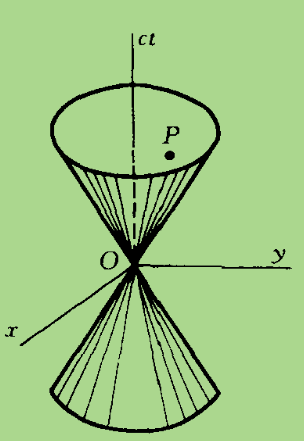
\includegraphics[width=6cm]{figure6-1.png}
    \caption{四维光锥}
    \label{figure6.1}
\end{wrapfigure}

    考虑这种分类的几何意义,我们可以使用四维光锥图来辅助理解\autoref{figure6.1}. 我们使用$P$点代表在这个时空中的一个事件,原点为另一个事件,则存在三种情况:
    \begin{itemize}
        \item 若事件$P$位于锥面上,则间隔$s^2 = 0$,和原点可以以光波方式进行联系,也成为了\textbf{类光间隔}
        \item 若事件$P$位于光锥内部,$s^2>0$,这被称为\textbf{类时间隔},可以通过低于光速的作用联系
        \item 若事件$P$位于光锥之外,$s^2<0$,这被称为\textbf{类空间隔},不可能与原点发生任何联系(除非存在高于光速的作用)
    \end{itemize}

\noindent 对于类时间隔,事件$P$位于原点的上、下半光锥的情况被称为\textbf{绝对未来}和\textbf{绝对过去},不同于只看时间得到的未来和过去,这时转换坐标系是不影响事件的先后顺序的。

    类时间隔中的上、下半光锥的绝对性体现了因果律。可以利用洛伦兹变换式证明。若存在两个事件$(x,t),(x^{\prime},t^{\prime})$,前者为原因,后者为结果,则根据洛伦兹变换式,可以得到
    \begin{equation}
        t_2^{\prime} - t_1^{\prime} = \frac{(t_2-t_1)-\frac{v}{c^2}(x_2-x_1)}{\sqrt{1-\frac{v^2}{c^2}}}
    \end{equation}

\noindent 若要保持因果关系绝对性,需要$t_2^{\prime} > t_1^{\prime}$,这意味着
\begin{equation}
    \left|\frac{x_2-x_1}{t_2-t_1}\right| < \frac{c^2}{v}
\end{equation}

\noindent 假设$|x_2-x_1| = u(t_2-t_1)$,其中$u$表示由原因到结果的作用传播速度,故
\begin{equation}
    uv<c^2
\end{equation}

\noindent 注意$u,v$均是在同一个坐标下的结果。这表明当不存在比光速更快的物体或者作用的时候,因果关系具有绝对性。注意这是宏观情况下的,在微观情况下量子力学可以导致因果关系不绝对(前提是承认定域性)。

    \subsubsection{同时相对性}
    对于类空间隔,不可能用任何方式联系(在目前的实验结果下),它们之间不存在因果关系,其先后次序也就失去了意义,用洛伦兹变换可以直接证明。设两事件$(x_1,t_1),(x_2,t_2)$间隔类空,则
    \begin{equation}
        |t_2-t_1| < \frac{1}{c} |x_2 - x_1|
    \end{equation}

\noindent 若在一个坐标系存在$t_2>t_1$,则在另一个参考系,得到
\begin{equation}
    t_2^{\prime} - t_1^{\prime} = \frac{(t_2-t_1)-\frac{v}{c^2}(x_2-x_1)}{\sqrt{1-\frac{v^2}{c^2}}}
\end{equation}

\noindent 当$v$足够大,总存在
\begin{equation}
    |t_2-t_1| = \frac{v}{c^2} |x_2-x_1|
\end{equation}

\noindent 使得
\begin{equation}
    t_2^{\prime}<t_1^{\prime}
\end{equation}

    特别地,如果速度$\overline{v}$满足
    \begin{equation}
        |t_2-t_1| = \frac{\overline{v}}{c^2} |x_2-x_1|
    \end{equation}

\noindent 则
\begin{equation}
    t_2^{\prime} = t_1^{\prime}
\end{equation}

    可见,具有类空间隔的两事件,时间次序的先后具有相对性。但这并没有什么问题,因为具有类空间隔的两事件无法发生联系,不存在因果关系,时间次序的先后或者同时都失去了同时意义。在不同地点同时发生的两事件不可能存在因果关系(可以证明这属于类空间隔),因此同时的概念必然是相对的。在一个坐标系下同时的两个事件在另一个坐标系下将会不同时。但注意,这不是说“同时”失去了意义,因为在同一个坐标系下,“同时”是存在的,只是在进行坐标变换的情况下,“同时”失去了意义。这个概念十分重要,它基本是相对论理论下的“时间延缓”和“尺度缩短”的根源。

    \subsubsection{运动时间的延缓}
    在不同参考系上观察统一过程,会发现时间间隔是不同的。对于一个特定的物体,取静止坐标系和运动坐标系(不存在绝对静止的坐标,所有的静止坐标都是对于特定物体而言的)$\sum$和$\sum^{\prime}$. 在静止坐标系下时间间隔
    \begin{equation}
        \Delta s^2 = c^2(t_2^2-t_1^2) =c^2 \Delta \tau^2
    \end{equation}

\noindent 在运动坐标系下,取$\Delta t=t_2^{\prime}-t_1^{\prime}$
\begin{equation}
    \Delta s^2 = c^2(t_2^{\prime}-t_1^{\prime})^2 - (x_2^{\prime}-x_1^{\prime}) = c^2 \Delta t^{2} - (\Delta x)^2
\end{equation}

\noindent 由时间不变性可得
\begin{equation}
    c^2 \Delta t^2 - (\Delta x)^2 = c^2 (\Delta \tau)^2
\end{equation}

\noindent 又$\frac{|\Delta x|}{\Delta t} = v$,所以
\begin{equation}
    \Delta t = \frac{\Delta \tau}{\sqrt{1-\frac{v^2}{c^2}}}
\end{equation}

\noindent 其中,$\Delta \tau$是静止坐标系中时间,被称为固有时。从某种意义上说,这个时间是绝对的(因为静止坐标系具有较为绝对的标准)。

    由于$\Delta t > \Delta \tau$,表示运动物体上所发生的自然过程比静止物体的同样过程延缓的,运动速度越大,延缓越严重。但请注意,\red{固有时是不会发生变化的}。这种效应是时空的基本属性引起的,与钟的具体结构无关。

    匀速运动下导致的时间延缓具有相对性,即存在互相延缓的情况,这源于不同坐标系的时钟无法对准,本质上是同时相对性。加速运动下将会导致绝对的物理效应,即一个坐标系下的运动时间会真的比另一个坐标系下的短,具体可参考“双生子谬论”。考虑星际航行的问题,虽然光速在宇宙尺度下显得很可怜,但临近光速时由于时间延缓效果,在静止参考系下计算要上万年、十万年的旅程实际上并不需要这么长,极端点到达光速的话将失去时间流逝,在自己的参考系下是瞬间达到宇宙任何地方的(当然要考虑宇宙膨胀的问题,如果膨胀速度大于或等于光速,有些地方将永远不可能到达),这给星系航行提供了可能。

    \subsubsection{运动尺度缩短}
    运动尺度缩短有这样的效应
    \begin{equation}
        l = l_0 \sqrt{1-\frac{v^2}{c^2}}
    \end{equation}

\noindent 其中$l_0$是在静止参考系下的长度,$v$是相对运动速度。长度缩短是相对的(即在这个参考系看来另一个参考系的物体长度缩短了,在那个参考系看来这个参考系的物体也缩短了),其源于同时性的相对性。我们定义一个物体的长度是在同一个参考系中运用同时性测量物体两端所在的事件点的间隔,而到了另一个参考系会发现同时性被打破了,这个时候时空间隔自然是不变的,但出现了时间间隔,因而空间间隔(也就是平时我们所说的长度)便发生了变化。总的来说,长度缩短是空间间隔发生了变化,根源是时空一体,时空间隔不变且坐标变换时同时的相对性。

    但需要注意的是,这个不同只是描述上的不同,在不同的参考系可以有不同的描述方法,但最后的物理结论是一致的。比如“飞车过峡谷”的问题,掉不掉落可以就放在静止参考系下看长度的关系(如果不考虑下落时间所带来的贡献的话),不用理会坐标系变换的“车短了还是峡谷短了”的问题,物理结论是不会发生变化的。

    \subsubsection{速度变换公式}
    由洛伦兹变换式可推出相对论的速度变换公式,设
    设
    \begin{equation}
        \left \{ \begin{aligned}
            &u_x = \frac{\dif x}{\dif t} \\
            &u_y = \frac{\dif y}{\dif t} \\
            &u_z = \frac{\dif z}{\dif t}
        \end{aligned} \right.
    \end{equation}

\noindent 为物体相对于$\sum$的速度,再令$\sum^{\prime}$相对于$\sum$沿着x轴以速度v运动(注意相比于之前的讨论,这里相当于有三个坐标系,除了可见的这两个还有物体本身的静止坐标系),则
\begin{equation}
    x^{\prime} = \frac{x-vt}{\sqrt{1-\frac{u_x-v}{1-\frac{v^2}{c^2}}}}, \quad t^{\prime} = \frac{t-\frac{v}{c^2}x}{\sqrt{1-\frac{v^2}{c^2}}}\label{equ6.4}
\end{equation}

\noindent 对\autoref{equ6.4}微分并相除可以得到x方向速度变换公式
\begin{equation}
    u^{\prime}_{x}=\frac{d x^{\prime}}{d t^{\prime}}=\frac{u_{x}-v}{1-\frac{v u_{x}}{c^{2}}}
\end{equation}

\noindent 同理得到另外两个方向的速度变换公式
\begin{equation}
\begin{aligned}u_{y}^{\prime}&=\frac{d y^{\prime}}{d t^{\prime}}=\frac{u_{y} \sqrt{1-\frac{v^{2}}{c^{2}}}}{1-\frac{v u_{x}}{c^{2}}} \\ u_{z}^{\prime}&=\frac{d z^{\prime}}{d t^{\prime}}=\frac{u_{z} \sqrt{1-\frac{v^{2}}{c^{2}}}}{1-\frac{v u_{x}}{c^{2}}}\end{aligned}
\end{equation}

\noindent 反变换式为
\begin{equation}
    u_{x}=\frac{u_{x}^{\prime}+v}{1+\frac{v u_{x}^{\prime}}{c^{2}}}, u_{y}=\frac{u_{y}^{\prime} \sqrt{1-\frac{v^{2}}{c^{2}}}}{1+\frac{v u_{x}^{\prime}}{c^{2}}}, u_{z}=\frac{u_{z}^{\prime} \sqrt{1-\frac{v^{2}}{c^{2}}}}{1+\frac{v u_{x}^{\prime}}{c^{2}}}
\end{equation}

    在$v \ll c,|u| \ll c$的时候即可过渡到经典的伽利略变换。

    \subsection{相对论理论的四维形式}
    \subsubsection{物理量按空间变换性质的分类}
    物理量可以分为标量、矢量、张量等类别,这种分类是依据物理量在空间转动下的变换性质来规定的。

    \paragraph{标量}
    有些物理量在空间中没有取向关系,这使得坐标系转动时,这些物理量保持不变。变换关系式为
    \begin{equation}
        u^{\prime} = u
    \end{equation}

    \paragraph{矢量}
    有些物理量在空间中有一定的取向性,会有一定量的分量表示,在作转动变换时,几个分量会按照同一方式变换。变换关系式88为
    \begin{equation}
        v_i^{\prime} = a_{ij} v_j
    \end{equation}

    \paragraph{二阶张量}
    有些物理量显示出更为复杂的空间取向性质,需要用两个矢量指标表示,共有九个分量(不同维度的空间不相同,九个分量是三维空间下的结果)。变换关系式为
    \begin{equation}
        T^{\prime}_{ij} = a_{ik} a_{jl} T_{kl}
    \end{equation}

\noindent 对称张量经过变换后依旧是对称的,反对称张量经过变换之后则依旧是反对称的。对称张量之迹(对角元素之和)是一个标量。

    可以根据有多少个自由指标判别属于哪一类物理量。

    \subsubsection{洛伦兹变换的思维形式}
    将时间作为第四个分量,为了保持量纲,令
    \begin{equation}
        x_4 = i c t
    \end{equation}

\noindent 洛伦兹变换是满足间隔不变性的变换,所以要保持
\begin{equation}
    x^{\prime}_u x^{\prime}_u = x_u x_u =C
\end{equation}

    洛伦兹变换可以视为四维空间的转动,坐标分量的变换关系为
    \begin{equation}
        x^{\prime}_u = \alpha_{uv}x_v
    \end{equation}

\noindent 沿着x轴匀速直线运动时的变换矩阵为
\begin{equation}
\alpha=\left[\begin{array}{cccc}{\gamma} & {0} & {0} & {\mathrm{i} \beta \gamma} \\ {0} & {1} & {0} & {0} \\ {0} & {0} & {1} & {0} \\ {-\mathrm{i} \beta \gamma} & {0} & {0} & {\gamma}\end{array}\right]
\end{equation}

\noindent 若取$x_4 - ct$,这样度规为$\operatorname{diag}(1,1,1,-1)$(不过感觉更为常用的形式是将时间那一项放到第一分量的位置的),由此得到的变换矩阵为
\begin{equation}
\alpha=\left[\begin{array}{cccc}{\gamma} & {0} & {0} & { \beta \gamma} \\ {0} & {1} & {0} & {0} \\ {0} & {0} & {1} & {0} \\ {- \beta \gamma} & {0} & {0} & {\gamma}\end{array}\right]
\end{equation}

    \subsubsection{四维协变量}
    协变量是指在洛伦兹变换下有确定的交换性质的量,包括标量、矢量和各阶张量。物理量都是协变量。注意协变量对应的变换关系式洛伦兹变换,所以必定是四维量才有可能是协变量。比如四维速度
    \begin{equation}
        v_u = \frac{\dif x_u}{\dif \tau}
    \end{equation}

\noindent 这里的$\tau$是固有时,不属于任何一个维度,取代了在三维运动学中的$t$的位置。

    电磁波中的相位
    \begin{equation}
        \phi = \vec{k} \cdot \vec{x} - \omega t
    \end{equation}
\noindent 也是协变量。这是因为其是对波峰通过时空点的计数,不随坐标系的变化而变化。由此可得到四维波矢量$k_u = (\vec{k},i \frac{\omega}{c})$,这也是协变量。

    \subsubsection{物理规律的协变性}
    如果一个方程的每一项属于同类协变量,在参考系变换下,每一项都按相同方式变换,结果保持方程形式不变。在参考系变换下方程形式不变的性质称为\textbf{协变性}。相对论原理要求一切惯性系都是等价的,在不同惯性系中物理规律表示为相同形式,这要求\red{表示物理规律的方程是协变的}。用数学表示即方程
    \begin{equation}
        F_u = G_u 
    \end{equation}

\noindent 经过洛伦兹变换形式不变
\begin{equation}
    F_u^{\prime} = G_u^{\prime}
\end{equation}

    \subsection{电动力学的相对论不变性}
    麦氏方程含有电荷密度$\rho$,电流密度$\vec{J}$,电场强度$\vec{E}$和磁感应强度$\vec{B}$. 下面对它们进行改写,使之能够满足四维协变性。

    \subsubsection{四维电流密度矢量}
    实验表明电荷是四维不变量,由于
    \begin{equation}
        Q = \int \rho \dif V
    \end{equation}

\noindent 容易知道,体积元在洛伦兹变换下会发生变化,这意味着电荷密度也会发生变化,为
\begin{equation}
    \rho = \frac{\rho_0}{\sqrt{1-\frac{u^2}{c^2}}} = \gamma_u \rho_0
\end{equation}
\noindent 其中$u$是相对速度。由此知道电流为
\begin{equation}
    \vec{J} = \rho \vec{u} = \gamma_u \rho \vec{u}
\end{equation}

    我们现在延展电流密度,引入其在四维空间的第四个分量
    \begin{equation}
        J_4 = i c \rho 
    \end{equation}
\noindent 得到 
\begin{equation}
    \vec{J}_u = \rho \vec{u}_u
\end{equation}

\noindent 其中$\vec{u}_u$是四维速度
\begin{equation}
    \vec{u}_u = \gamma_u(\vec{u},ic)
\end{equation}

\noindent 由此得到电流密度的四维矢量
\begin{equation}
    \vec{J}_u = (\vec{J},ic\rho)
\end{equation}

\noindent 由此可见$\vec{J}$和$\rho$的统一性。粒子运动带来的效果是两者的协变,两者在四维框架下应该视为同一物理量的不同方面,从经典视角下便是空间依赖项和时间依赖项。由此对于电荷守恒可以改写成四维形式
\begin{equation}
    \frac{\partial J_u}{\partial x_u} = 0 \qquad u =1,2,3,4
\end{equation}

\noindent 显然具有协变性。

    \subsubsection{四维势矢量}
    使用洛伦兹规范,得到运动方程
    \begin{equation}
        \left \{ \begin{aligned}
            &\nabla^2 \vec{A} - \frac{1}{c^2} \frac{\partial^2 \vec{A}}{\partial t^2} = -\mu_0 \vec{J}  \\
            &\nabla^2 \varphi - \frac{1}{c^2} \frac{\partial^2 \varphi }{\partial t^2} = - \frac{\rho}{\varepsilon_0}
        \end{aligned} \right.
    \end{equation}

\noindent 得到规范条件
\begin{equation}
    \nabla \cdot \vec{A} + \frac{1}{c^2} \frac{\partial \varphi }{\partial t} = 0
\end{equation}

    考虑四维下的微分算符
    \begin{equation}
        \bigcirc^2 = \nabla^2 - \frac{1}{c^2}\frac{\partial^2}{\partial t^2} = \frac{\partial}{\partial x_u}\frac{\partial}{\partial x_u}
    \end{equation}

\noindent 所以得到
\begin{equation}
    \left \{ \begin{aligned}
        &\bigcirc^2 \vec{A}  = - \mu_0 \vec{J} \\ 
        & \bigcirc^2 \varphi = - \mu_0 c^2 \rho 
    \end{aligned} \right.
\end{equation}

\noindent 由此可见,$\vec{A}$和$\varphi$也可以合为一个四维势矢量
\begin{equation}
    A_u = (\vec{A},\frac{i}{c}\varphi)
\end{equation}

\noindent 则
\begin{equation}
    \bigcirc A_u = - \mu_0 J_u
\end{equation}

\noindent 也具有明显的协变性。除此之外,我们发现,对于洛伦兹条件可以写成
\begin{equation}
    \frac{\partial A_u}{\partial x_u} = 0
\end{equation}

\noindent 也具有协变性。 

    在参考系变换下,四维势按矢量进行变换
    \begin{equation}
        A_u^{\prime} = \alpha_{u v} A_v
    \end{equation}

\noindent 若参考系$\sum^{\prime}$相对于$\sum$沿着x方向以速度$v$运动,根据四维变换矩阵
\begin{equation}
\alpha=\left[\begin{array}{cccc}{\gamma} & {0} & {0} & {\mathrm{i} \beta \gamma} \\ {0} & {1} & {0} & {0} \\ {0} & {0} & {1} & {0} \\ {-\mathrm{i} \beta \gamma} & {0} & {0} & {\gamma}\end{array}\right]
\end{equation}

\noindent 得到
\begin{equation}
    \left \{ \begin{aligned}
        &A_x^{\prime} = \gamma\left(A_x-\frac{v}{c^2} \varphi\right) \\
        &A_y^{\prime} = A_y \\ 
        &A_z^{\prime} = A_z \\ 
        &\varphi^{\prime} = \gamma\left(\varphi - v A_x\right)
    \end{aligned} \right.
\end{equation}

    \subsubsection{电磁场张量}
    对于
    \begin{equation}
        \left \{ \begin{aligned}
            &\vec{B}= \nabla \times \vec{A} \\
            &\vec{E} = - \nabla \varphi - \frac{\partial \vec{A}}{\partial t}
        \end{aligned} \right.
    \end{equation}

\noindent 可以发现其分量都由$\left(\frac{\partial A_v}{\partial x_u} - \frac{\partial A_u}{\partial x_v}\right)$ 构成,不妨引入一个反对称四维张量
\begin{equation}
    F_{uv} = \left(\frac{\partial A_v}{\partial x_u} - \frac{\partial A_u}{\partial x_v}\right)
\end{equation}

\noindent 由此得到一个重要的四维张量——电磁场张量
\begin{equation}
F_{\mu v}=\left[\begin{array}{cccc}{0} & {B_{3}} & {-B_{2}} & {-\frac{\mathrm{i}}{c} E_{1}} \\ {-B_{3}} & {0} & {B_{1}} & {-\frac{\mathrm{i}}{c} E_{2}} \\ {B_{2}} & {-B_{1}} & {0} & {-\frac{\mathrm{i}}{c} E_{3}} \\ {\frac{\mathrm{i}}{c} E_{1}} & {\frac{\mathrm{i}}{c} E_{2}} & {\frac{\mathrm{i}}{c} E_{3}} & {0}\end{array}\right]
\end{equation}

    利用电磁场张量可以改写麦克斯韦方程组
    \begin{equation}
        \left \{ \begin{aligned}
            &\nabla \cdot \vec{E} = \frac{\rho}{\varepsilon_0} \\ 
            &\nabla \times \vec{B} = \mu_0 \varepsilon_0 \frac{\partial \vec{E}}{\partial t}+ \mu_0 \vec{J}
        \end{aligned} \right. \rightleftharpoons \frac{\partial F_{u v}}{\partial x_v} = \mu_0 J_u
    \end{equation}

\noindent 和
\begin{equation}
    \left \{ \begin{aligned}
        &\nabla \cdot \vec{B} =0 \\ 
        &\nabla \times \vec{E} = - \frac{\partial \vec{B}}{\partial t} 
    \end{aligned} \right. \rightleftharpoons \frac{\partial F_{uv}}{\partial x_{\lambda}}+\frac{\partial F_{v\lambda}}{\partial x_u}+\frac{\partial F_{\lambda u}}{\partial x_v} = 0
\end{equation}

    由动量变换关系
    \begin{equation}
        F_{uv}^{\prime} = \alpha_{u\lambda} \alpha_{v\tau} F_{\lambda \tau}
    \end{equation}

\noindent 导出电磁场的变换关系
\begin{equation}
\begin{array}{c}{E_{1}^{\prime}=E_{1}, \quad B_{1}^{\prime}=B_{1}} \\ {E_{2}^{\prime}=\gamma\left(E_{2}-v B_{3}\right), \quad B_{2}^{\prime}=\gamma\left(B_{2}+\frac{v}{c^{2}} E_{3}\right)} \\ {E_{3}^{\prime}=\gamma\left(E_{3}+v B_{2}\right), \quad B_{3}^{\prime}=\gamma\left(B_{3}-\frac{v}{c^{2}} E_{2}\right)}\end{array}
\end{equation}

\noindent 写为更为对称的形式
\begin{equation}
\begin{array}{l}{\vec{E}_{/ /}^{\prime}=\vec{E}_{/ /}, \quad \vec{B}_{/ /}^{\prime}=\vec{B}_{/ \prime}} \\ {\vec{E}_{\perp}^{\prime}=\gamma(\vec{E}+\vec{v} \times \vec{B})_{\perp}, \quad \vec{B}_{\perp}^{\prime}=\gamma\left(\vec{B}-\frac{\vec{v}}{c^{2}} \times \vec{E}\right)_{\perp}}\end{array}
\end{equation}

\noindent 其中的平行、垂直符号表明的是和相对运动速度平行、垂直的分量。

    通过对匀速v运动的带电荷e的粒子的电磁场进行分析,会发现在坐标系变换后磁场“无中生有”。但其实这就说明了磁场其实是一种相对论效应,本质上还是电场。电磁现象由此得到统一。

    \subsubsection{电磁场的不变量}
    用指标收缩,得到有电磁场张量$F_{uv}$构成洛伦兹不变量
    \begin{equation}
        \frac{1}{2} F_{uv} F^{uv} = B^2 - \frac{1}{c^2} E^2\label{equ6.5}
    \end{equation}

\noindent 还可以构造另一个洛伦兹不变量,为此引入四维全反对称张量$\varepsilon_{uv\lambda\tau}$,定义为
\begin{equation}
    \varepsilon_{uv\lambda\tau}  \left \{ \begin{aligned}
        &= +1,\qquad \text{偶次变换可得到1234} \\
        &= -1,\qquad \text{奇次变换可得到1234} \\
        &= 0,\qquad \ \ \ \text{任意两个指标一样} 
    \end{aligned} \right.
\end{equation}

\noindent 由张量变换性质
\begin{equation}
    \varepsilon_{uv\lambda\tau}^{\prime} = \alpha_{ua}\alpha_{v\beta}\alpha_{\lambda r} \alpha_{\tau \delta}\varepsilon_{a\beta r \delta} = (\operatorname{Det} \varepsilon_{uv\lambda\tau})=\varepsilon_{uv\lambda\tau}
\end{equation}

\noindent 可见满足协变性。利用全反对称张量,可以由电磁场张量构造另一不变量
\begin{equation}
    \frac{i}{8}\varepsilon_{uv\lambda\tau} F_{uv} F_{\lambda \tau} = \frac{1}{c} \vec{B} \cdot \vec{E}\label{equ6.6}
\end{equation}

    真空中有
    \begin{equation}
        |\vec{B}| = \frac{\vec{E}}{c} , \vec{B} = \frac{1}{c} \vec{n} \times \vec{E}
    \end{equation}

\noindent 所以对于这两个不变量\autoref{equ6.5}和\autoref{equ6.6}都为0.而且这两个性质还是与坐标无关的。

    \subsection{相对论力学}
    略
    \subsection{从作用量出发串联起相对论电动力学}
    \subsubsection{作用量}
    电磁场的作用量如下
    \begin{equation}
        I \int \dif t \dif V \left(-\frac{1}{4} F_{uv} F^{uv} + \mu_0 J^{u} A_u\right)
    \end{equation}

\noindent 通过对$\vec{A}$求变分,可以得到运动方程
\begin{equation}
    \partial_u F^{uv} = - \mu_0 J^{v}
\end{equation}

\noindent 由于$F^{uv}$是反对称矩阵,等价于$\partial_v F^{uv} = \mu_0 J^u$.

    作用量还可以改写为度规表示
    \begin{equation}
        I = \int \sqrt{g} \dif x^4 \left(-\frac{1}{4} F_{uv} F^{uv} + \mu_0 J^{u} A_u\right)
    \end{equation}

    \subsubsection{对称性}
    作用量有以下对称性
    \begin{itemize}
        \item 作用量是洛伦兹不变量 $\Rightarrow$ 运动方程是协变的
        \item 电磁对偶性质不变
        \begin{equation}
            F^{uv} \rightarrow i^{*} F^{uv} = \frac{i}{2}\varepsilon^{uv\rho \sigma}F_{\rho \sigma}
        \end{equation}
        \item 共形变换不变
        \item 规范变换不变
    \end{itemize}

    \subsubsection{动量流密度张量}
    \begin{equation}
       T = - \varepsilon_0 \left(\vec{E} \vec{E} - \frac{1}{2} I E^2\right) - \frac{1}{\mu_0}\left(\vec{B}\vec{B} - \frac{1}{2} I B^2\right)
    \end{equation}
\end{document}
